%%%%%%%%%%%%%%%%%%%%%%%%%%%%%%%%%%%%%%%%
%%% DOCUMENT CLASS AND CLASS OPTIONS %%%
%%%%%%%%%%%%%%%%%%%%%%%%%%%%%%%%%%%%%%%%

% Initial authors:     Michael Enders, Felix Lammermann
% Author's emails:     latex@flammermann.de
%
% Current maintainers: Markus Putnings
% Maintainer's emails: markus.putnings@fau.de
%
%
% Copyright 2019--2020 Michael Enders & Felix Lammermann
% 
% This work may be distributed and/or modified under the conditions of the
% LaTeX Project Public License, either version 1.3c of this license or (at your
% option) any later version.
% 
% The latest version of this license is in
% 
%   http://www.latex-project.org/lppl.txt
% 
% and version 1.3c or later is part of all distributions of LaTeX version
% 2008-05-04 or later.
% 
% This work has the LPPL maintenance status `maintained'.
% The current maintainer of this work is Markus Putnings.

\documentclass[
  paper = 17x24,
    % 17x24 (= studienpartitur, default)
    % a5 (= a5paper)
  language = english,
    % german (= default)
    % english
  acronym = split,
    % none (= false)
    % split (= true, default)
    % combined
    % onlyabbreviation (= nosymbol)
    % onlysymbol (= noabbreviation)
  acronymline = novertical,
    % none (= false)
    % both (= true, all, default)
    % onlyhorizontal (= novertical)
    % onlyvertical (= nohorizontal)
  %TODO fix faupress bibliography
  bibliography = false,
    % none (= false)
    % split (= true, default)
    % combined
  %TODO fix faupress bibliography
  bibliographypart = false,
    % none (= false)
    % all (= true, default)
    % onlymain
    % nomain
    % onlyown
    % noown
    % onlystudent
    % nostudent
  titlesize = Huge,
    % Huge (= default)
    % LARGE
    % Large
    % large
    % normalsize
  par = halfskip,
    % skip
    % halfskip (= default)
    % indent
]{faupress}


%%%%%%%%%%%%%%%%%%%%%%%%%%%
%%% INDIVIDUAL PACKAGES %%%
%%%%%%%%%%%%%%%%%%%%%%%%%%%
\usepackage{amsmath}
\usepackage{amssymb}
\usepackage{blindtext}
\usepackage{physics}
\usepackage{bm}
\usepackage{relsize}
\usepackage{amsthm}
\theoremstyle{definition}
\newtheorem{theorem}{Theorem}
\newtheorem{definition}{Definition}
\usepackage{caption}
\usepackage{subcaption}
\usepackage{graphicx}
\usepackage{algorithmicx}
\usepackage{algorithm}
\usepackage{algpseudocode}
\usepackage{tikz}
\newcommand{\ps}[1]{\langle #1 \rangle}
\newcommand{\bps}[1]{ \ps{\bm{#1}} }

%%%%%%%%%%%%%%%%%
%%% META INFO %%%
%%%%%%%%%%%%%%%%%

% publication
\title{Evolving Efficient Multigrid Methods with Grammar-Guided Genetic Programming}
%\subtitle{Subtitle}

% author
\firstname{Jonas}
\lastname{Schmitt}
\degree{M.Sc.}
\origin{Forchheim}

% publication identifiers
\yearofpublication{Year of Publication}
\series{}
\volume{XXX}
\doi{10.25593/978-3-96147-XXX-X}
\isbn{978-3-96147-XXX-X}
\eisbn{978-3-96147-XXX-X}
\issn{2625-9974}
\printinformation{%
  ggf. Satz \\%
  ggf. Druck%
}

% miscellaneous
\subject{Doktorarbeit}
\keywords{FAU, Erlangen, Nürnberg, Doktorarbeit}

% university and examination
\institute{Lehrstuhl für Informatik 10}
\supervisor{Prof. Harald Köstler}
\oralexam{Date of oral exam}
\dean{Vorsitzender Pruefungskommision}
\reviewer{%
}


%%%%%%%%%%%%%%%%%%%%%%%%%
%%% DOCUMENT CONTENTS %%%
%%%%%%%%%%%%%%%%%%%%%%%%%

\begin{document}

% typeset the titlepage of the publisher
\maketitle

% start the frontmatter (roman page numbering,
% lowercase roman sectioning numbering, no header)
\frontmatter
  
  % typesets the titlepage of the faculty
  \makefacultytitle

  % insert preface heading (has \label{ch:preface},
  % reference via \nameref{ch:preface})
  \begin{preface}
   
    %%% WRITE YOUR PREFACE DIRECTLY HERE OR %%%%%%%%
    %%% INPUT AN EXTERNAL FILE WITH YOUR PREFACE %%%
    %\blindtext

    
  \end{preface}

  % typeset the table of contents
  \tableofcontents

  % typeset the list of symbols and/or abbreviations,
  % settings can be tweaked via the two class options
  % acronym and acronymlist
  \faupressprintacronyms
  
  % typeset the list of figures
  \listoffigures
  
  % typeset the list of tables
  \listoftables

% start the mainmatter (arabic page numbering [reset],
% arabic sectioning numbering, header)
\mainmatter

  % inserts introduction heading (hat \label{ch:intro},
  % reference via \autoref{ch:intro} or \ref{ch:intro})
\chapter{Introduction}
    
    %%% WRITE YOUR INTRODUCTION DIRECTLY HERE OR %%%%%%%%
    %%% INPUT AN EXTERNAL FILE WITH YOUR INTRODUCTION %%%
    %\blindtext


\chapter{Background}
  %%% WRITE YOUR THESIS DIRECTLY HERE OR %%%%%%
  %%% INPUT EXTERNAL FILES WITH YOUR THESIS %%%
  \section{Discretization of Partial Differential Equations}\label{sec:discretization}
Many problems in science and engineering can be modeled as partial differential equations (PDEs). %TODO insert references
A PDE is an equation that contains functions of one or multiple variables together with their partial derivatives.
Consider, for instance, the equation
\begin{equation}
	-\alpha \nabla^2 u = f \quad \text{in} \; \Omega 
	\label{eq:heat-equation}
\end{equation}
where $u = u(\bm{x})$ and $f = f(\bm{x})$ are both functions with respect to the vector of space variables $\bm{x} = (x_1, x_2, \dots, x_n)^T$ and $\Omega \supset \mathbb{R}^d$.
Equation~\eqref{eq:heat-equation} describes the temperature distribution inside a medium whose thermal conductivity is determined by the coefficient $\alpha$ and which contains a heat source $f$.
Since Equation~\eqref{eq:heat-equation} is only satisfied in the interior of the domain $\Omega$, we, additionally need to define a set of conditions at its boundaries.
These so-called \emph{boundary conditions} (BCs) can be usually classified in four different types:
\begin{description}
	\item[Dirichlet] $u(\bm{x}) = g(\bm{x})$
	\item[Neumann] $\frac{\partial}{\partial \vec{n}} u(\bm{x}) = 0$
	\item[Robin] $a u(\bm{x}) + b \frac{\partial}{\partial \vec{n}} u(\bm{x}) = g(\bm{x})$
	\item[Cauchy] $a u(\bm{x}) = g(\bm{x}), \; b \frac{\partial}{\partial \vec{n}} u(\bm{x}) = h(\bm{x})$
\end{description}
Here $\frac{\partial}{\partial \vec{n}} u(\bm{x})$ denotes the partial derivative of $u$ with respect to outwards-directed normal vector of the boundary.
Note that the difference between Robin and Cauchy BCs is that in the former case one condition is formulated as a weighted average of $u$ and its derivative in normal direction, while for the latter two conditions must be met individually.
While depending on the boundary conditions an analytical solution for Equation~\eqref{eq:heat-equation} might exist, for many PDEs such a solution has not been discovered or its computation is unfeasible.
A remedy is the application of so-called numerical methods, that are based on approximating the solution of a given PDE on a discrete set of grid points. 
\subsection{Grid Creation}
Before computing a numerical approximation of the solution of a given PDE, we need to define a set of discrete points within the domain $\Omega$ at which we aim to obtain the solution.
Usually, these points are defined on a grid or mesh with certain structure.
In general, a distinction is made between structured (or regular) and unstructured grids.
A structured grid is characterized by the uniform neighborhood of its grid points, which means that the number of neighbors is typically the same for each grid point.
In contrast, each point within an unstructured grid can have a varying number of neighbors.
Computations are usually easier to implement and more efficient on structured grids, due to their regularity.
However, structured grids are often difficult to create on complicated and irregular domains.
On the other hand, unstructured grids offer a higher degree of flexibility and are, therefore, also well-suited for the previously mentioned cases. %TODO include references
This thesis focuses on numerical methods that can be formulated on a hierarchy of structured grids. 
In the following, we, therefore, focus on this particular grid type.
One possibility to approximate a given PDE on a structured set of grid points is to compute the Taylor series expansion around each of them points, which leads to the so-called \emph{finite difference method} (FDM).
\subsection{Finite Difference Method}
For the sake of simplicity, we consider the one-dimensional function $u(x)$.
To obtain an approximation for the derivatives of $u$, we can compute its Taylor expansion in the neighborhood of $x$ with a step size $h$, which yields
\begin{equation}
	u(x + h) = u(x) - h \dv{x} u(x) + \mathcal{O}(h^2)
\end{equation}
Assuming $h$ is sufficiently small, the first-order approximation 
\begin{equation}
	\dv{x} u(x) \approx \frac{u(x + h) -  u(x)}{h}
\end{equation}
is obtained.
Furthermore, we can derive an approximation for the second-order partial derivative $\dv[2]{x}$ by considering
\begin{equation}
	u(x + h) = u(x) + h \dv{x} u(x) + \frac{h^2}{2} \dv[2]{x} u(x) + \mathcal{O}(h^3)
	\label{eq:taylor-forward}
\end{equation}
and 
\begin{equation}
	u(x - h) = u(x) - h \dv{x} u(x) + \frac{h^2}{2} \dv[2]{x} u(x) + \mathcal{O}(h^3).
	\label{eq:taylor-backward}
\end{equation}
Adding Equation~\eqref{eq:taylor-backward} to Equation~\eqref{eq:taylor-forward} then yields the second-order finite difference approximation
\begin{equation}
	 \dv[2]{x} u(x) \approx \frac{u(x + h) + u(x - h) - 2u(x)}{h^2}.
\end{equation}
Using the same technique similar approximation terms can be obtained for higher-dimensional functions and higher-order derivatives. %TODO Referenz einfügen
While finite differences offer a simple and straightforward way to approximate a given PDE on a set of structured grid points, in many cases the underlying physical requirements and complex geometries necessitate the use of semi-structured or even unstructured grids together more complicated approaches such as the finite volume (FVM) and finite element method (FEM) together with the use of semi- or unstructured grids.
For an in-depth introduction to these methods, the reader is referred to one of the following references:
%TODO insert references about FVM and FEM
\subsection{Model Problem}
To illustrate the previous two sections, we consider the following model problem, which represents a two-dimensional version of Poisson's equation:
\begin{equation}
	\begin{split}
		-\frac{\partial^2}{\partial x^2} u(x,y) - \frac{\partial^2}{\partial y^2} u(x,y) & = f(x, y) \quad \forall x, y \in (0, 1) \\
		u(0, y) = u(x, 0) = u(1, y) = u(x, 1) & = 0 \quad \forall x, y \in (0, 1)
	\end{split}
	\label{eq:2D-poisson-model}
\end{equation}
Note that this equation corresponds to the two-dimensional steady-state heat equation with constant $\alpha = 1$ on the unit square $\Omega = ( 0, 1 )^2$.
We then discretize Equation~\eqref{eq:2D-poisson-model} using finite differences and a uniform step size $h$, which yields
\begin{equation}
	\begin{split}
		\frac{1}{h^2} (4 u_{i,j} - u_{i-1, j} - u_{i+1, j} - u_{i, j-1} - u_{i, j+1}) & = f_{i, j} \quad \forall i, j \in \{1, 2, \dots n\} \\
		u_{0, j} = u_{i, 0} = u_{n+1, j} = u_{i, n+1} & = 0 \quad \forall i, j \in \{1, 2, \dots n\}
	\end{split} 
	\label{eq:2D-poisson-model-discrete}
\end{equation}
with $u_{i,j} = u(ih, jh)$, $f_{i,j} = f(ih, jh)$ and $n = 1/h - 1$.
By defining a unique ordering of the grid points $u_{i, j}$, Equation~\eqref{eq:2D-poisson-model-discrete} we can be transformed to a system of linear equation of type $A \bm{u} = \bm{f}$. 
For instance, setting $h = 0.25$, results in $n = 3$ and, hence, a total number of nine grid points.
%TODO draw grid
Assuming a natural ordering of grid points, we can represent the resulting system of linear equations as follows
\begin{equation}
\frac{1}{h^2} \underbrace{ \begin{pmatrix}
\begin{array}{ccc|ccc|ccc}~4&-1&~0&-1&~0&~0&~0&~0&~0\\-1&~4&-1&~0&-1&~0&~0&~0&~0\\~0&-1&~4&~0&~0&-1&~0&~0&~0\\\hline -1&~0&~0&~4&-1&~0&-1&~0&~0\\~0&-1&~0&-1&~4&-1&~0&-1&~0\\~0&~0&-1&~0&-1&~4&~0&~0&-1\\\hline ~0&~0&~0&-1&~0&~0&~4&-1&~0\\~0&~0&~0&~0&-1&~0&-1&~4&-1\\~0&~0&~0&~0&~0&-1&~0&-1&~4\end{array}
	\end{pmatrix}}_{\textstyle A}
\underbrace{
	\begin{pmatrix}
	u_{11} \\ u_{12} \\ u_{13} \\ u_{21} \\ u_{22} \\ u_{23} \\ u_{31} \\ u_{32} \\ u_{33}
\end{pmatrix}}_{\textstyle{\bm{u}}} = \bm f
\label{eq:2D-poisson-assembled-matrix}
\end{equation}
with a right-hand side $\bm f$, which can be further reduced with respect to the given boundary conditions that assume a constant value of zero at all boundary points:
\begin{equation}
\bm f = \begin{pmatrix}
		f_{11} + \frac{1}{h^2} (u_{10} + u_{01}) \\f_{12} + \frac{1}{h^2} u_{02} \\ f_{13} + \frac{1}{h^2} (u_{03} + u_{14})  \\ f_{21} + \frac{1}{h^2} u_{20} \\ f_{22} \\ f_{23} + \frac{1}{h^2} u_{24} \\ f_{31} + \frac{1}{h^2} (u_{30} + u_{41}) \\ f_{32} + \frac{1}{h^2} u_{42} \\ f_{33} + \frac{1}{h^2} (u_{34} + u_{43})
\end{pmatrix} = \begin{pmatrix}
f_{11} \\
f_{12} \\ 
f_{13} \\ 
f_{21} \\ 
f_{22} \\
f_{23} \\
f_{31} \\ 
f_{32} \\
f_{33}
\end{pmatrix}.
\label{eq:2D-poisson-assembled-rhs}
\end{equation}
Note that $A$ represents a sparse matrix, which means that only a minority of its entries are nonzero.
Moreover, since we already represent the solution of Equation~\ref{eq:2D-poisson-model-discrete} on a regular grid, storing the resulting linear system in a matrix-vector format is inefficient.
If we assume that each operation required for solving a system of linear equations can be formulated in form of a matrix-vector or vector-vector operation, it is unnecessary to store the corresponding matrix explicitly.
Instead, we only have to store the computational pattern that corresponds to a matrix-vector multiplication performed on a vector with the respective ordering of the grid points.
On regular grids, each of such pattern can be represented as a so-called stencil code.
\subsection{Stencil Codes}
\label{subsec:stencil-codes}
In general, a stencil code can be considered as a set of mappings from an n-dimensional index vector to a complex-valued number.
More formally we can define the general stencil $S^{(m,d)}$ as a finite set of $m$ tuples of the following form:

\begin{equation}
	\begin{split}
			& S^{(m, d)} = \{(\bm{a}_k, b_k) \}_{k=1}^m = \{(\bm{a}_1, b_1),  (\bm{a}_2, b_2), \dots (\bm{a}_m, b_m)\} 
	\\ & \forall \, i, j, k \in \{1, 2, \dots m \}: \,
	\bm{a}_k \in \mathbb{Z}^d \wedge \bm{a}_i \neq \bm{a}_j \; \text{with} \; i \neq j, \; b_k \in \mathbb{C}.
	\end{split}
\end{equation}
Here, the left entry $\bm{a}_k$ of each tuple $(\bm{a}_k, b_k)$ denotes the \emph{offset} from the index of the current grid point and the left entry $b_k$ the respective \emph{weight} or \emph{value}.
For one- and two-dimensional problems, it is often more convenient to use the alternative notation 
\begin{equation}
	S^{(m, 1)} = \begin{bmatrix}
		\cdots & s_{-1} & s_{0} & s_{1} & \cdots
	\end{bmatrix}
\end{equation}
and
\begin{equation}
	S^{(m, 2)} = \begin{bmatrix}
		& \vdots & \vdots & \vdots & \\
		\cdots & s_{1,-1} & s_{1,0} & s_{1,1} & \cdots \\
		\cdots & s_{0,-1} & s_{0,0} & s_{0,1} & \cdots \\
		\cdots & s_{-1,-1} & s_{-1,0} & s_{-1,1} & \cdots \\
		& \vdots & \vdots & \vdots &
	\end{bmatrix}
\end{equation}
where for all $s_{\bm{a}_i}$  with $i \in \{1, \dots, m\}$ there exists a tuple $(\bm{a}_i, b_i) \in S^{(m, d)}$ such that $b_i = s_{\bm{a}_i}$.
We can also extend this notation to three dimensions, by representing all components with the same offset as a separate two dimensional stencil, such that
\begin{equation}
	S^{(m,3)} = 
	\begin{bmatrix}
		\cdots & S_{z-1}^{(m_{z-1},2)} & S_{z}^{(m_{z},2)} & S_{z+1}^{(m_{z+1},2)} & \cdots 
	\end{bmatrix},
\label{eq:3D-stencil-matrix-notation}
\end{equation}
where $m = \sum_{i} m_{z+i}$.
%TODO specify range of i

Furthermore, we define the application of a stencil $S^{(m, d)}$ to a certain point $u_{\bm i}$ with $\bm i \in \mathcal G$, where $\mathcal G \supset \mathbb{N}^d$ is the set of grid indices, each considered as an n-dimensional vector:
\begin{equation}
	\begin{split}
		& S^{(m, d)} \bullet u_{\bm i} = \sum_{k=1}^m b_k u_{\bm i + \bm{a}_k} \quad 
		\text{with} \; \bm{i} \in \mathcal G \supset \mathbb{N}^d, \\ & (\bm{a}_i, b_i) \in S^{(m,d)} \; \forall \, i \in \{ 1, 2, \dots m \} 
	\end{split}
\label{eq:stencil-application}
\end{equation}
For $d = 3$, we can formulate the application of a three-dimensional stencil $S^{(m,3)}$, based on Equation~\eqref{eq:3D-stencil-matrix-notation}, as a dot product of the form
\begin{equation}
	S^{(m, 3)} \bullet u_{x,y,z} = 	
\begin{bmatrix}
	\cdots & S_{z-1}^{(m_{z-1},2)} & S_{z}^{(m_{z},2)} & S_{z+1}^{(m_{z+1},2)} & \cdots 
\end{bmatrix} \bullet
\begin{bmatrix}
	\vdots \\ u_{x,y,z-1} \\ u_{x,y,z} \\ u_{x,y,z+1} \\ \vdots 
\end{bmatrix},
\end{equation}
where each element-wise multiplication is interpreted as an application of the operator defined in Equation~\eqref{eq:stencil-application}.

As a two-dimensional example we consider the following five-point stencil:
\begin{equation}
	\begin{split}
		\Delta_h^{(5,2)} = & \bigg\{ \left( \left( 0,0 \right), \frac{4}{h^2}\right), \left(\left(1,0\right), \frac{-1}{h^2}\right), \left(\left(-1,0\right), \frac{-1}{h^2}\right), \\ & \left(\left(0,1\right), \frac{-1}{h^2}\right), \left(\left(0,-1\right), \frac{-1}{h^2}\right) \bigg\}
	\end{split}
	\label{eq:five-point-stencil}
\end{equation}
Applying $\Delta_{h}^{(5,2)}$ to a given point $u_{i,j}$ on a two-dimensional regular grid yields 
\begin{equation}
	\Delta_h^{(5,2)} \bullet u_{i,j} = \frac{1}{h^2} \left(4 u_{i+0,j+0}  - u_{i-1,j+0} - u_{i+1,j+0} - u_{i+0,j-1} - u_{i+0,j-1}\right),
\end{equation}
which corresponds precisely to the left part of Equation~\eqref{eq:2D-poisson-model-discrete}.
From this example it becomes evident that applying a given stencil to set of points $u_{\bm x}$ defined on a regular grid can be always considered as a sparse matrix-vector product, where the matrix is obtained by sorting the grid points according to a well-defined order, which has been already demonstrated in Equation~\eqref{eq:2D-poisson-assembled-matrix}.
Therefore, in case it is possible to define each computational step for solving a given discretized PDE on a regular grid by means of a stencil application, we only need to obtain the respective stencil entries instead of assembling or even storing a complete matrix.
Furthermore, many operators defined for matrices can be easily transferred into the domain of stencil codes.
As a first elementary operation, we define the multiplication of a stencil with a scalar, which is simply achieved by multiplying the weight of each entry with the respective value:
% Scalar multiplication
\begin{equation}
	\alpha S^{(m, d)} = \{(\bm{a}_k, \alpha b_k) \}_{k=1}^m
\end{equation}

Next, we can define certain binary operations such as the addition, subtraction and multiplication of two stencils.
Equation~\eqref{eq:stencil-addsub} contains a recursive definition of stencil addition and subtraction.
Here, we simply add the weights of each entry with the same offset contained in both $S_1$ and $S_2$.
In case an offset is not contained in both stencils the respective tuple is included unmodified.  
% Stencil addition and subtraction
\begin{equation}
	S_1 \pm S_2 = 
	\begin{cases}
		\{(\bm{a}, b\pm c ) \} \cup (\tilde{S}_1 \pm \tilde{S}_2) & \text{if} \; S_1 = 	\{(\bm{a}, b ) \} \cup \tilde{S}_1 \\
		& \text{and} \; S_2 = \{(\bm{a}, c ) \} \cup \tilde{S}_2 \\
		
		\{(\bm{a}, b ) \} \cup (\tilde{S}_1 \pm S_2) & \text{if} \; S_1 = 	\{(\bm{a}, b ) \} \cup \tilde{S}_1 \\
		& \text{and} \; \{(\bm{a}, c ) \} \notin S_2 \;
		\forall c \in \mathbb{C}
		\\
% TODO case probably unnecessary
%		\{(\bm{a}, c ) \} \cup (S_1 \pm \tilde{S}_2) & \text{if} \; S_2 = 	\{(\bm{a}, c ) \} \cup \tilde{S}_2 \wedge
%		\{(\bm{a}, b ) \} \notin S_1 \; \forall b \in \mathbb{C}
%		\\
		S_1 & \text{if} \; S_2 = \emptyset
		\\
		S_2 & \text{else} 
		\\
	\end{cases}
\label{eq:stencil-addsub}
\end{equation}
Based on Equation~\eqref{eq:stencil-addsub} we can then also provide a definition of the multiplication of two stencils $S_1$ and $S_2$, which can be seen as a recursive version of the iterative computation scheme described in~\cite{rittich2018extending}:
% Stencil multiplication
\begin{equation}
	S_1 \cdot S_2 = 
	\begin{cases}
		\{(\bm{a} + \bm{\hat{a}}, b \cdot \hat{b} ) \} +  \{(\bm{a}, b ) \} \cdot \tilde{S}_2 + \tilde{S}_1 \cdot S_2 & \text{if} \; S_1 = \{(\bm{a}, b ) \} \cup \tilde{S}_1 \\
		&
		\text{and} \; S_2 = \{(\bm{\hat{a}}, \hat{b} ) \} \cup \tilde{S}_2 \\
		\emptyset & \text{if} \; S_1 = \emptyset \vee S_2 = \emptyset
	\end{cases}
\label{eq:stencil-mult}
\end{equation}
Here, to compute the stencil product $S_1 \cdot S_2$, for each pair of entries $\{(\bm{a}, b ) \} \in S_1$ and $\{(\bm{\hat{a}}, \hat{b} ) \} \in S_2$ the tuple $\{(\bm{a} + \bm{\hat{a}}, b \cdot \hat{b} ) \}$ needs to be formed.
To define this computation recursively, we first pick random entries $\{(\bm{a}, b ) \} \in S_1$ and $\{(\bm{\hat{a}}, \hat{b} ) \} \in S_2$ and combine them as described above.
We then multiply the entry $\{(\bm{a}, b ) \}$ chosen from $S_1$ with the remainder stencil $\tilde{S}_2 = S_2 \setminus \{(\bm{\hat{a}}, \hat{b} ) \}$, which means that we now obtain the combination of this entry with all remaining ones from $S_2$.
Finally, the process is continued recursively by computing the product of the remainder $\tilde{S}_1 = S_1 \setminus \{(\bm{a}, b ) \}$, with the original stencil $S_2$.
Since it is possible that the combination of different pairs of stencil offsets leads to the same result, we, additionally, need to sum up the corresponding weights and combine them in a single tuple.
For this purpose, we employ stencil addition, as defined in Equation~\eqref{eq:stencil-addsub}, to sum up all tuples with matching offset obtained within each recursive subcomputation.
%TODO introduce array stencil notation for 1D and 2D
\subsection{Systems of Partial Differential Equations}
While so far we have only considered problems formulated in form of a single partial differential equation, many phenomena can only be modeled in form of a system of PDEs.
One of the most simple systems of PDEs is the so-called biharmonic equation
\begin{equation}
	\begin{split}
		\nabla^2 u & = v  \\
		\nabla^2 v & = f.
	\end{split}
\label{eq:biharmonic-system}
\end{equation}
As a remark, note that this system is mathematically equivalent to the scalar equation 
\begin{equation}
	\nabla^4 u = f.
\end{equation}
We can reformulate Equation~\eqref{eq:biharmonic-system} to obtain
\begin{equation}
	\underbrace{
	\begin{pmatrix}
		\nabla^2 & -1 \\
		0 & \nabla^2
	\end{pmatrix}}_{A}
\underbrace{ 
	\begin{pmatrix}
		u \\ v
	\end{pmatrix}
}_{\bm{u}}
=
\underbrace{
\begin{pmatrix}
	0 \\ f
\end{pmatrix}
}_{\bm{f}}.
\label{eq:biharmonic-system-matrix-formulation}
\end{equation}
While in contrast to our previous examples Equation~\eqref{eq:biharmonic-system-matrix-formulation} includes partial derivatives of multiple variables, we can employ the same techniques to discretize each individual operator and obtain a corresponding system of linear equations. 
Consider the two-dimensional biharmonic system
\begin{equation}
	\begin{split}
		\frac{\partial^2}{\partial x^2} u(x,y) + \frac{\partial^2}{\partial y^2} u(x,y) - v(x, y) & = 0 \\
		\frac{\partial^2}{\partial x^2} v(x,y) + \frac{\partial^2}{\partial y^2} v(x,y) & = f(x, y) \\ \forall x, y \in (0, 1)^2
	\end{split}
	\label{eq:2D-biharmonic-system}
\end{equation}
Discretizing Equation~\eqref{eq:2D-biharmonic-system} using finite differences with a uniform step size $h$ and rewriting the resulting equations in stencil form yields
\begin{equation}
		\begin{pmatrix}
			\Delta_h^{(5,2)} & -1 \\
			0 & \Delta_h^{(5,2)}
	\end{pmatrix}
		\begin{pmatrix}
			u_{i,j} \\ v_{i,j}
		\end{pmatrix}
	=
		\begin{pmatrix}
			0 \\ f_{i,j}
		\end{pmatrix} \\
\forall i,j \in \{1, 2, \dots n\},
	\label{eq:2D-biharmonic-system-stencil}
\end{equation}
where $\Delta_h^{(5,2)}$ is the two-dimensional five-point stencil defined in Equation~\eqref{eq:five-point-stencil}.
Equation~\eqref{eq:2D-biharmonic-system-stencil} then represents a system of two linear equations which needs to be solved at every pair of grid points $u_{i,j}$ and $v_{i,j}$.
If we consider Equation~\eqref{eq:2D-biharmonic-system-stencil} at all grid points at once, a system of linear equations is obtained whose solution corresponds to the discrete solution of Equation~\eqref{eq:2D-biharmonic-system}.
Before we conclude this section, it is important to mention that we have not yet discussed how each variable, in the given case $u_{i,j}$ and $v_{i,j}$, is placed on the grid.
While it is tempting to always place each variable at the same position within a grid, in many applications this leads to undesirable numerical properties.%TODO insert reference
As a consequence, often more complex grid placing strategies are used in practice, for instance so-called staggered grids, which we, for the sake of brevity, do not discuss here.
For a detailed treatment of these techniques, the reader is referred to %TODO insert suitable reference
.
Also note that in order to solve Equation~\eqref{eq:2D-biharmonic-system}, or any other system of PDEs, we need to define suitable conditions at the boundaries of each domain on which a given variable, contained in one of the equations, is defined.
These boundary conditions can be of the same type as described above.
Again, for a more detailed treatment of boundary conditions for systems of PDEs, the reader is referred to %TODO insert suitable reference
.
 



  \section{Basic Iterative Methods}~\label{section:basic-iterative-methods}
In general, the methods for solving systems of linear equations can be assigned to two categories: Direct and iterative methods.
Direct methods are characterized by the fact that they are able to compute the exact solution of a linear system in a finite number of steps.
In contrast, iterative methods are based on computing a series of approximations for the solution of the linear system.
Even though this series often converges to the exact solution, there is usually no guarantee that the approximations will ever reach the accuracy of a solution computed by a direct method.
Unfortunately, for many problems applying direct methods infeasible, due to their high computational complexity and memory storage requirements.
For instance, Gaussian elimination, in general, requires $\mathcal O(n^3)$ operations for solving a system of linear equations with $n$ unknowns.
Moreover, since the goal of Gaussian elimination is to transform a given matrix into upper-triangular form, it based on the direct manipulation of the input matrix and, hence, usually requires storing it explicitly.
In contrast, many iterative methods are exclusively based on the computation of matrix-vector products and, hence, do not require to manipulate the input matrix directly.
As we have shown in Section~\ref{subsec:stencil-codes}, the discretization of many partial differential equations enables the representation of matrix-vector products as the application of a stencil code, whereas each stencil is directly derived from the discretization of a continuous differential operator.
If we assume that each stencil includes only a finite number of entries and that we need to store at most one stencil per grid point, we can reduce the storage requirements to $\mathcal{O}(n)$, where $n$ is the total number of grid points.
In case the same stencil applies to the whole domain, we even only need to store a single stencil, whose memory requirements are negligible compared to those for storing each grid point.
Furthermore, due to the approximation of real numbers by floating-point numbers on a computer, even the solution of a direct method is prone to numerical errors.
As a consequence, in practice, the exactness of direct methods is often undermined by these effects and, hence, the approximations computed by an iterative method can achieve the same degree of numerical accuracy.%TODO include ref
Furthermore, assuming that we can compute an acceptable approximation using only a finite number of $m$ matrix-vector multiplications, the application of an iterative method reduces the computational complexity for solving a system of linear equations to $O(mn)$.
In the following, we first introduce basic iterative methods, as the Jacobi and Gauss-Seidel method, and then derive fundamental statements about their convergence. 
%Finally, as multigrid methods represent the fundamental basis for this work, we discuss these methods in greater detail.   
\subsection{Jacobi and Gauss-Seidel} 
We begin our introduction of basic iterative methods by considering the general system of linear equations
\begin{equation}
	A \bm{x} = \bm{b},
	\label{eq:general-system-of-linear-equations}
\end{equation}
where $A$ is the coefficient matrix, $\bm x$ the vector of unknowns and $\bm b$ the right-hand side.
At this point we do not specify whether $A$ represents a dense/sparse matrix or a stencil, as long as all the operations employed within the subsequent methods are well-defined for a mathematical object of this type.
We can now rewrite Equation~\eqref{eq:general-system-of-linear-equations} to obtain
\begin{equation}
	\bm{x} = \bm{x} + \bm b - A \bm{x}.
	\label{eq:general-fixed-point}
\end{equation}
Which can be considered a fixed point of the form
\begin{equation}
	\bm x = f(\bm x).
\end{equation} 
Replacing $\bm x$ by $\bm{x}^{(k+1)}$ in the left and by $\bm{x}^{(k)}$ in the right part of Equation~\eqref{eq:general-fixed-point} yields the fixed-point iteration
\begin{equation}
	\bm{x}^{(k+1)} = \bm{x}^{(k)} + \bm b - A \bm{x}^{(k)}.
	\label{eq:richardson-iteration}
\end{equation}
Equation~\eqref{eq:richardson-iteration} is usually called Richardson iteration and can be considered as the most basic form of an iterative method for solving a system of linear equations.
Here, the term $\bm{r}^{(k)} = \bm{b} - A \bm{x}^{(k)}$ represents the \emph{residual} or \emph{defect} in iteration $k$ of the method.
Next, we consider 
\begin{equation}
	M^{-1} A \bm{x} = M^{-1} \bm{b},
	\label{eq:general-preconditioned-system-of-linear-equations}
\end{equation}
which represents a modified version of Equation~\eqref{eq:general-system-of-linear-equations}, that is obtained by multiplying each side of the equation by the inverse of a matrix $M$.
By the rules of linear algebra, Equation~\eqref{eq:general-preconditioned-system-of-linear-equations} is equivalent to the original system and therefore has the same solution.
However, it can be also considered as a left-preconditioned version of Equation~\eqref{eq:general-system-of-linear-equations}, with $M$ as preconditioner.
By, again, considering the fixed point of Equation~\eqref{eq:general-preconditioned-system-of-linear-equations} we obtain the iteration
\begin{equation}
	\bm{x}^{(k+1)} = \bm{x}^{(k)} + M^{-1}(\bm b - A \bm{x}^{(k)}),
	\label{eq:general-stationary-iterative-method}
\end{equation}
which represents the general form of a stationary iterative method. 
For instance, if we replace $M$ with the unit matrix $I$, we obtain a Richardson iteration.
Furthermore, setting $M = A$ allows us to obtain the solution in one step since then
\begin{equation}
	\bm{x}^{(k+1)} = \bm{x}^{(k)} + A^{-1}(\bm b - A \bm{x}^{(k)}),
	\label{eq:one-step-iteration}
\end{equation}
which leads to
\begin{equation}
	\bm{x}^{(k+1)} = A^{-1}\bm b.
\end{equation}
The result of this iteration $x^{(k+1)}$ is hence independent of the choice of $x^{(k)}$ and if we insert $A^{-1}\bm b$ Equation~\eqref{eq:general-system-of-linear-equations} it becomes apparent that this term always represents the correct solution of the respective system of linear equations.
Since the computation of the inverse of a general matrix $A$, in general, is more expensive and numerically unstable than solving the system directly, the application of Equation~\eqref{eq:one-step-iteration} is impracticle.
However, with it we can already provide an intuition about the choice of $M$.
The closer $M^{-1}$ is to the actual inverse of $A$, the faster the convergence of the respective stationary iterative method will usually be.
In contrast, the choice of a matrix $M$ that is easy to invert, where the Richardson iteration represents a extreme case with $I^{-1} = I$, leads to an iterative method that is easy to compute, but potentially suffers from slow convergence.
Before we introduce some basic iterative methods that fall into this framework, note that we can reformulate Equation~\eqref{eq:general-stationary-iterative-method} to obtain
\begin{equation}
	M (\bm{x}^{(k+1)} - \bm{x}^{(k)}) = \bm{b} - A \bm{x}^{(k)}. 
\end{equation}
Moreover, by defining $\bm{c}^{(k+1)}$ as the correction term
\begin{equation}
	\bm{c}^{(k+1)} = \bm{x}^{(k+1)} - \bm{x}^{(k)},
\end{equation}
we obtain a new system of linear equations
\begin{equation}
	M \bm{c}^{(k+1)} = \bm{b} - A \bm{x}^{(k)}. 
	\label{eq:general-stationary-iterative-method-system-formulation}
\end{equation}
The solution of this system $\bm{c}^{(k+1)}$ then provides us with the approximate solution in step $i+1$ through the relation
\begin{equation}
	\bm{x}^{(k+1)} =  \bm{x}^{(k)} + \bm{c}^{(k+1)}.
\end{equation}
To obtain a new approximate solution in every iteration, we can, therefore, solve the system of linear equations denoted by Equation~\eqref{eq:general-stationary-iterative-method-system-formulation}, instead of computing the inverse of $M$.

Since, as we have already mentioned, it is desirable to choose $M \approx A$, we define the splitting
\begin{equation}
	A = D - L - U,
\end{equation} 
where $D$ is the lower diagonal, $-L$ the lower triangular and $-U$ the upper triangular part of $A$, respectively.
Both the Jacobi as well as the Gauss-Seidel method are defined based on this splitting.
First of all, setting $M = D$, yields the Jacobi method
\begin{equation}
	\bm{x}^{(k+1)} = \bm{x}^{(k)} + D^{-1}(\bm b - A \bm{x}^{(k)}).
	\label{eq:jacobi-method}
\end{equation}
Note that since $D$ is a diagonal matrix, we can easily obtain its inverse by inverting all its diagonal entries.
Therefore, each iteration of the Jacobi method consists of a simple matrix-vector multiplication of the residual $\bm{r}^{(k)} = \bm{b} - A \bm{x}^{(k)}$ with the diagonal matrix $D^{-1}$.
To define the Jacobi method in the domain of stencil codes with respect to our derivation presented in Section~\ref{subsec:stencil-codes}, we need to obtain the diagonal of a given stencil $S$.
As an offset of zero in each dimension always refers to the grid point on which the stencil is applied and therefore to the diagonal entry in each line of the corresponding matrix.
We can therefore define the diagonal of $S$ as
\begin{equation}
	\text{diag}(S) = \begin{cases}
		\{(\bm{0}, b) \} & \text{if} \; (\bm 0, b) \in S \\
		\emptyset & \text{else}.
	\end{cases}
	\label{eq:stencil-diag}
\end{equation}
Based on this definition, we can also specify the inverse diagonal of a stencil as
\begin{equation}
	\text{diag-inv}(S) = \begin{cases}
		\{(\bm{0}, \frac{1}{b}) \} & \text{if} \; (\bm 0, b) \in S \\
		\emptyset & \text{else}.
	\end{cases}
	\label{eq:stencil-diag-inv}
\end{equation}
Because the Jacobi method, as defined in Equation~\eqref{eq:jacobi-method}, does often suffer from slow convergence, it is common to introduce a \emph{relaxation factor} or \emph{weight} $\omega$, which leads to the so-called weighted Jacobi method
\begin{equation}
	\bm{x}^{(k+1)} = \bm{x}^{(k)} + \omega D^{-1}(\bm b - A \bm{x}^{(k)}),
	\label{eq:weighted-jacobi-method}
\end{equation}
where $\omega$ is chosen from the interval $\left(0, 2\right)$.
Here, a value of $\omega$ smaller than one is usually called underrelaxation, while for a value greater than one the term overrelaxation is used.
Note that $\omega = 1$ leads to the original Jacobi method without any relaxation.

Next, we define the Gauss-Seidel method with $M = D - U$ which results in an iteration of the form
\begin{equation}
	(D - L) \bm{c}^{(k+1)} = \bm{b} - A \bm{x}^{(k)}, 
	\label{eq:gauss-seidel-method}
\end{equation}
where, again, $\bm{c}^{(k+1)}$ is the correction term $\bm{c}^{(k+1)} = \bm{x}^{(k+1)} - \bm{x}^{(k)}$.
Note that since $M = D - L$ does not represent a diagonal matrix, we can not easily obtain its inverse, but instead solve Equation~\eqref{eq:gauss-seidel-method} in each iteration of the method.
As $D - L$ is a lower triangular matrix, the solution of this system can be computed with a single step of back substitution. 
To apply the Gauss-Seidel method within the domain of stencil codes, we also need to define a function that extracts the lower triangle of a given stencil.
As each diagonal entry corresponds to an offset of zero in each dimension, we can obtain the lower triangle by only including all entry with an offset lower than zero.
The resulting operation is defined in Equation~\eqref{eq:stencil-lower}.
\begin{equation}
	\text{lower}(S) = \begin{cases}
		\{(\bm{a}, b) \} \cup \text{lower}(\tilde{S}) & \text{if} \; \exists\, \bm a, b \; \text{with} \; \bm a < \bm 0 \; \text{and} \; S = (\bm a, b) \cup \tilde{S} \\
		\text{lower}(\tilde{S}) & \text{if} \; \exists\, \bm a, b \; \text{with} \; \bm a \geq \bm 0 \; \text{and} \; S = (\bm a, b) \cup \tilde{S} \\
		\emptyset & \text{else}.
	\end{cases}
	\label{eq:stencil-lower}
\end{equation}

Similarly, we can also provide a definition for obtaining the upper triangle of a given stencil, which is formulated in Equation~\eqref{eq:stencil-upper}.
\begin{equation}
	\text{upper}(S) = \begin{cases}
		\{(\bm{a}, b) \} \cup \text{upper}(\tilde{S}) & \text{if} \; \exists\, \bm a, b \; \text{with} \; \bm a > \bm 0 \; \text{and} \; S = (\bm a, b) \cup \tilde{S} \\
		\text{upper}(\tilde{S}) & \text{if} \; \exists\, \bm a, b \; \text{with} \; \bm a \leq \bm 0 \; \text{and} \; S = (\bm a, b) \cup \tilde{S} \\
		\emptyset & \text{else}.
	\end{cases}
	\label{eq:stencil-upper}
\end{equation}
While there are many more iterative methods that can be formulated in the form of Equation~\eqref{eq:general-stationary-iterative-method}, the goal of this section is to introduce only those concepts necessary for a basic understanding of these method's functioning.
Therefore, we postpone the treatment of other and more advanced variants of the methods presented here to later chapters of this thesis. 

\subsection{Convergence}
In contrast to direct methods, which compute the solution of a given system of linear equations in a fixed number of computational steps, iterative methods compute a series of approximations.
The method is then said to convergence when the difference between the actual solution and subsequent approximations approaches zero.
To quantify this behavior, we introduce a number of metrics used for evaluating the quality of a series of approximations obtained through a specific iterative method.
First of all, we can define the error in iteration $k$ as
\begin{equation*}
	\bm{e}^{(k)} = \bm{x}^{(k)} - \bm{x}^{*},
\end{equation*}
where $\bm{x}^{(k)}$ is the $k$th approximation and $\bm{x}^{*}$ the correct solution of the system.
While the error gives as an immediate way to quantify the accuracy of an approximation, we usually do not know the correct solution of a given system of linear equations and therefore are not able to compute this metric.
As a remedy, we can instead consider the residual
\begin{equation*}
	\bm{r}^{(k)} = \bm{b} - A \bm{x}^{(k)},
\end{equation*}
which can be always computed irrespective of whether the solution of the system is known.
Note that the residual will be always zero in case the error is zero.
We then reconsider that the iterative methods introduced in the last section can be all considered a fixed-point iteration of the form
\begin{equation}
	\bm{x}^{(k+1)} = \bm{x}^{(k)} + M^{-1}(\bm b - A \bm{x}^{(k)}),
\end{equation}
and assume that $\bm{e}^{(k)} = \bm{0}$.
Hence, we have $\bm{x}^{(k)} = \bm{x}^{*}$ and the above equation is reduced to
\begin{equation}
	\bm{x}^{(k+1)} = \bm{x}^{*}.
\end{equation}
The solution $\bm{x}^{*}$ of the system $A \bm{x} = b$ is therefore a fixed point of each stationary iterative method.
However, note that this represents a necessary and not a sufficient condition. 
We, therefore, consider an arbitrary fixed-point of Equation~\eqref{eq:general-stationary-iterative-method}
\begin{equation*}
	\bm{x} = \bm{x} + M^{-1}(\bm b - A \bm{x}).
\end{equation*}
Transforming this equation again into a system of linear equations yields
\begin{equation*}
	M^{-1} A \bm{x} = M^{-1}\bm b,
\end{equation*}
which means that each fixed-point $\bm{x}$ represents a solution of the preconditioned linear system~\eqref{eq:general-preconditioned-system-of-linear-equations} and, hence, also of the original system~\eqref{eq:general-system-of-linear-equations}.
If we assume that $A$ is a square, nonsingular matrix, the solution of each system of linear equations with $A$ as its coefficient matrix is unique and, therefore, it must be true that $\bm{x} = \bm{x}^{*}$.
After we have ensured that in case a stationary iterative method has converged to a fixed-point $\bm{x}$, it is equal to the correct solution of the linear system the method aims to solve.
However, the question remains to be answered under which conditions a sequence of the form of Equation~\eqref{eq:general-stationary-iterative-method} converges to a fixed point and how many iteration must be performed to achieve this goal.
For this purpose, we, again, reformulate Equation~\eqref{eq:general-stationary-iterative-method} to obtain
\begin{equation}
	\bm{x}^{(k+1)} = (I - M^{-1} A) \bm{x}^{(k)} + M^{-1}\bm b,
\end{equation}
as an alternative formulation.
Within this equation can now set $\bm{x}^{i} = \bm{x}^{0}$ 
\begin{equation}
	\bm{x}^{(1)} = (I - M^{-1} A) \bm{x}^{(0)} + M^{-1}\bm b,
\end{equation}
and expand this sequence to the two-iteration series
\begin{equation}
	\bm{x}^{(2)} = (I - M^{-1} A)^2 \bm{x}^{(0)} + (2I - M^{-1} A)M^{-1} \bm{b}.
\end{equation}
By continuing this recursively for an arbitrary number of $k$ times, we see that the resulting equation will always be of the form
\begin{equation}
	\bm{x}^{(k)} = (I - M^{-1} A)^k \bm{x}^{(0)} + N^{(k)}\bm{b},
	\label{eq:stationary-iterative-method-series}
\end{equation}
which means that we can always separate the term $N^{(k)}\bm{b}$ from the rest of the equation.
Note that here the superscript $G^k$ means that we have the $k$th power of $G$, while $N^{(k)}$ means that the matrix has been obtained through $k$ recursive substitutions of the respective iterate $\bm{x}^{(k)}$.
Since we have obtained Equation~\eqref{eq:stationary-iterative-method-series} from our original formulation it still holds true that $\bm{x}^{*}$ is a fixed point of this sequence and, thus, subtracting by $\bm{x}^{*}$ yields
\begin{equation}
	\bm{x}^{(k)} - \bm{x}^{*} = (\underbrace{I - M^{-1} A}_{G})^k (\bm{x}^{(0)} - \bm{x}^{*}).
	\label{eq:iteration-matrix-sequence}
\end{equation}
Here, $G = I - M^{-1} A$ is the so-called \emph{iteration matrix} of the given stationary iterative method.
Before we reason about convergence of this sequence, we introduce the spectral radius 
\begin{equation}
	\rho (A)=\max \limits_{1 \leq k \leq n} |\lambda _{k}|,
\end{equation}
where $A$ is a matrix of rank $n$ with the eigenvalues $\lambda_{1}, \dots, \lambda_{n}$.
Based on this definition we can then state the following theorem:
\begin{theorem}
$\lim \limits_{k \to  \infty} G^k = 0$ if and only if $\rho(G) < 1$.
\label{theorem:general-convergence-result}
\end{theorem}
%TODO potentially prove theorem

While Theorem~\ref{theorem:general-convergence-result} provides an answer whether the sequence~\eqref{eq:iteration-matrix-sequence} converges to zero, we still do not have any knowledge about the speed of this process.
For this purpose, we introduce the general \emph{convergence factor} $\rho$ of a sequence of the form of Equation~\eqref{eq:iteration-matrix-sequence} as
\begin{equation}
	\rho = \lim \limits_{k \to  \infty} \left( \max \limits_{x^{(0)} \in \mathbb{R}^{n}} \frac{\norm{\bm{x}^{(k)} - \bm{x}^{*}}}{\norm{\bm{x}^{(0)} - \bm{x}^{*}}} \right)^{\frac{1}{k}}.
\end{equation} 
Furthermore, the \emph{convergence rate} $\tau$ is defined as the natural logarithm of the inverse of the convergence factor
\begin{equation}
	\tau = -\ln \rho
\end{equation}
\begin{theorem}
	$\rho = \rho(G)$.
	\label{theorem:convergence-factor}
\end{theorem}
%TODO potentially prove theorem
\begin{proof}
	For a proof of Theorem~\ref{theorem:general-convergence-result} and~\ref{theorem:convergence-factor} the reader is referred to ~\cite{varga1962iterative,saad2003iterative}.
\end{proof}
As a result of Theorem~\ref{theorem:convergence-factor} we can state that the spectral radius $\rho(G)$ gives a lower limit for the speed of convergence of every stationary iterative method with an iteration matrix $G = I - M^{-1} A$ that is independent of the choice of the initial vector $\bm{x}^{(0)}$.
Since stationary iterative methods are all based on the simple formulation in Equation~\eqref{eq:general-stationary-iterative-method}, they are both easy to implement and analyze.
The application of these methods alone, however, leads to slow convergence in solving many PDE-based problems~\cite{briggs2000multigrid}.
While many other iterative methods for solving the systems of linear equations arising from the discretization of PDEs have been formulated~\cite{saad2003iterative}, the main focus of this thesis is on multigrid method, which will be discussed in the following section.



  \section{Multigrid Methods}\label{sec:multigrid-methods}
%Multigrid methods aim to accelerate the convergence of iterative methods by eliminating certain error components more efficiently on a coarser resolution of the same problem.
While basic iterative methods, such as Jacobi and Gauss-Seidel, are applicable to many PDE-based problems, in practice, their speed of convergence is often insufficient, which means that a large number of iterations is required until an acceptable approximation accuracy can be attained. 
The main reason for this behavior is that these methods are only efficient in the reduction of certain error components, while others remain mostly unaffected~\cite{briggs2000multigrid}.
This can be best understood by investigating their effect on oscillatory errors with different frequencies.
For this purpose, we consider the one-dimensional Laplace equation
\begin{equation}
		\begin{split}
			- \Delta u(x) & = 0 \quad \forall x \in (0, 1) \\
			u(0) & = u(1) = 0,
		\end{split}
		\label{eq:1D-laplace-model}
\end{equation}
which is discretized using the three-point stencil
\begin{equation}
	- \Delta_h = \frac{1}{h^2}\begin{bmatrix}
		-1 & 2 & -1
	\end{bmatrix}.
		\label{eq:1D-laplace-stencil}
\end{equation} 
Figure~\ref{fig:different-error-components} shows the impact of applying the Jacobi and Gauss-Seidel method to different periodic error components.
\begin{figure}
	\centering
	\begin{subfigure}[t]{0.32\textwidth}
		\centering
		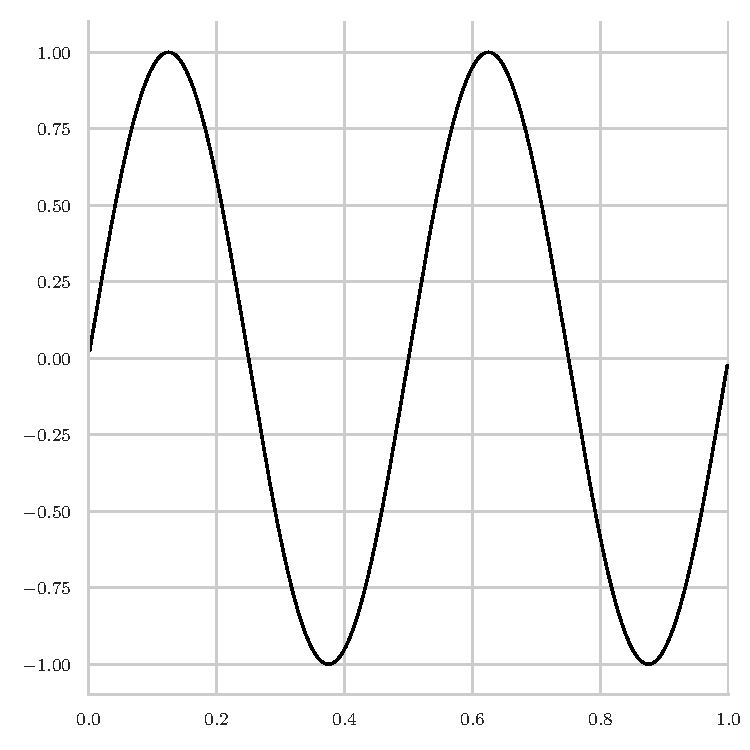
\includegraphics[width=\textwidth]{figures/error_plots//initial_error_jacobi_4pi.pdf}
		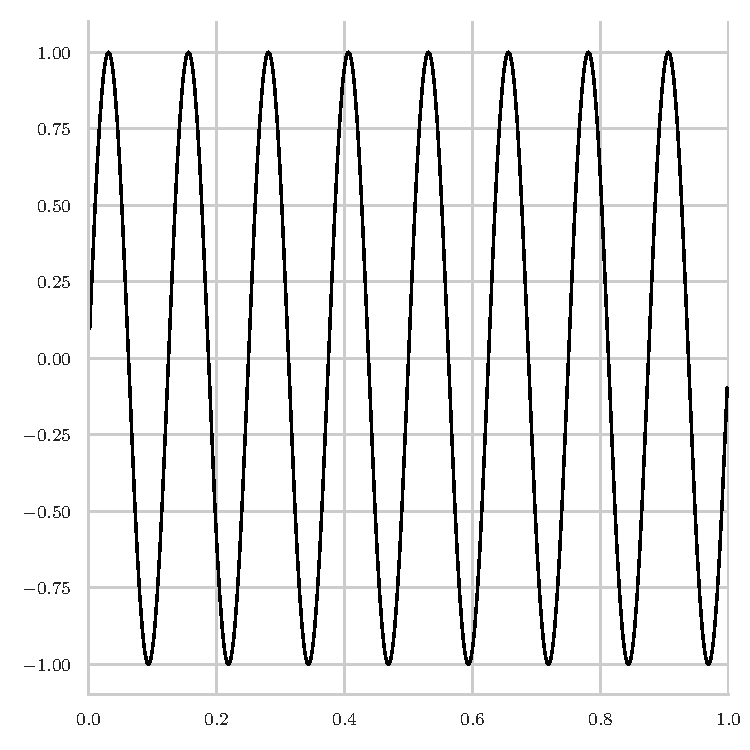
\includegraphics[width=\textwidth]{figures/error_plots//initial_error_jacobi_16pi.pdf}
		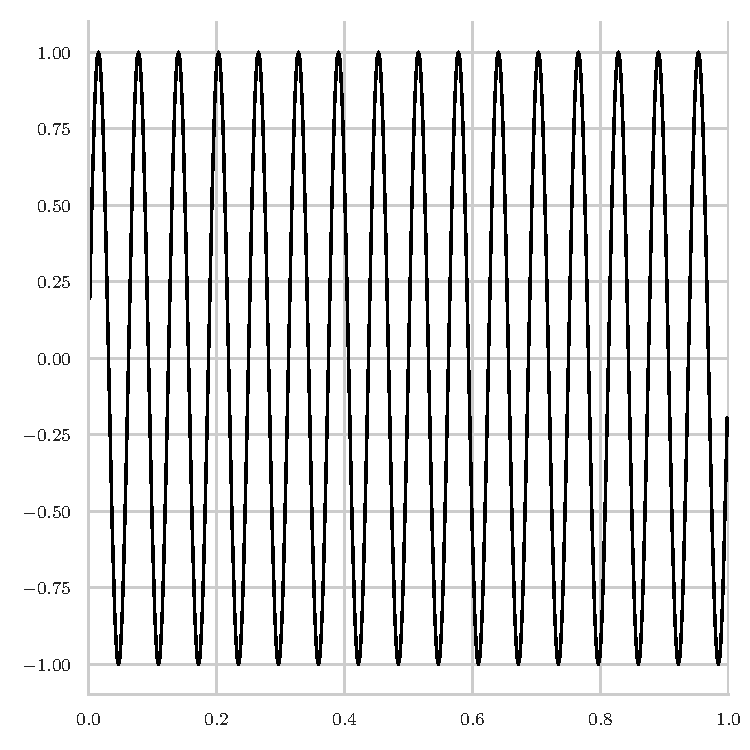
\includegraphics[width=\textwidth]{figures/error_plots//initial_error_jacobi_32pi.pdf}
		\caption{Initial error}
	\end{subfigure}
	\hfill
	\begin{subfigure}[t]{0.32\textwidth}
		\centering
		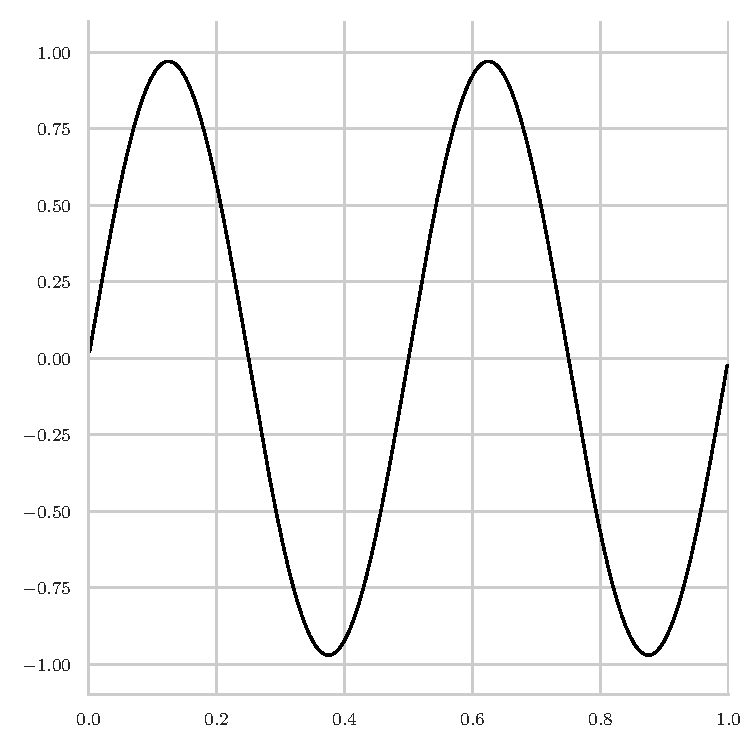
\includegraphics[width=\textwidth]{figures/error_plots//final_error_jacobi_4pi.pdf}
		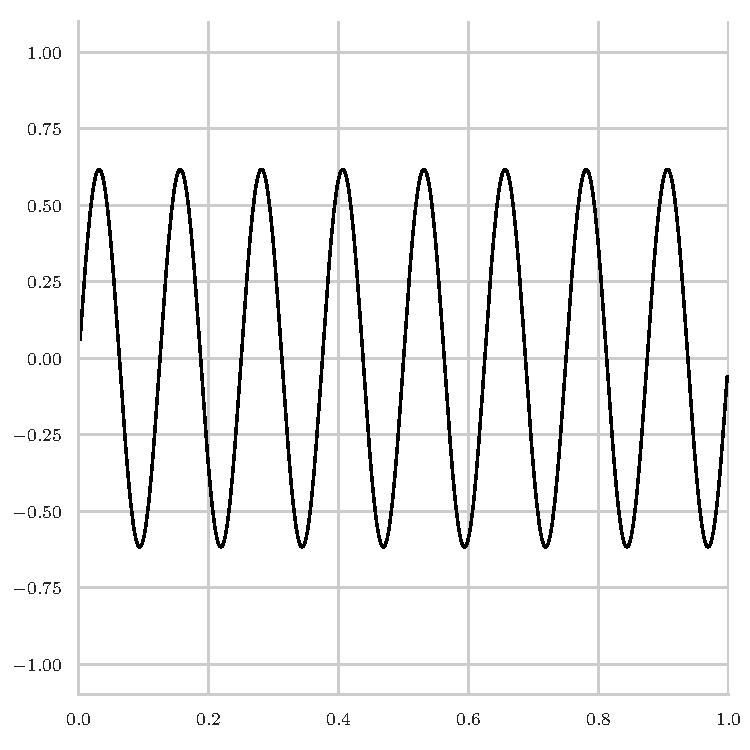
\includegraphics[width=\textwidth]{figures/error_plots//final_error_jacobi_16pi.pdf}
		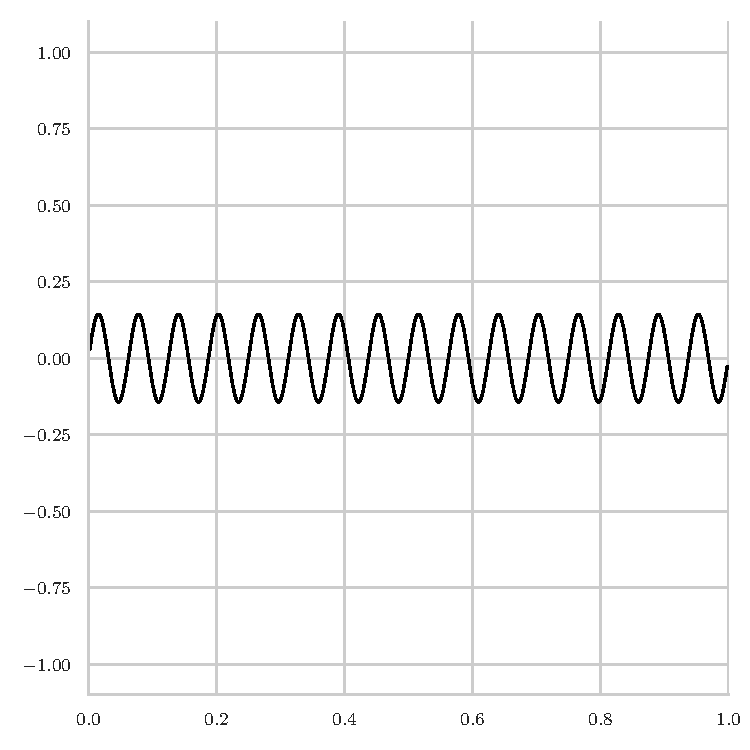
\includegraphics[width=\textwidth]{figures/error_plots//final_error_jacobi_32pi.pdf}
	\caption{Error after applying Jacobi}
	\end{subfigure}
	\hfill
	\begin{subfigure}[t]{0.32\textwidth}
		\centering
		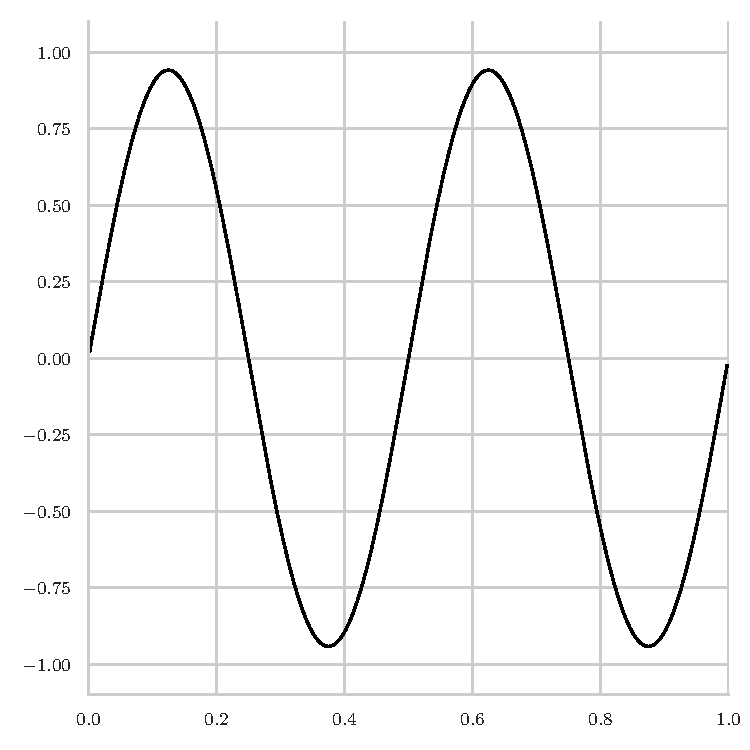
\includegraphics[width=\textwidth]{figures/error_plots//final_error_gauss_seidel_4pi.pdf}
		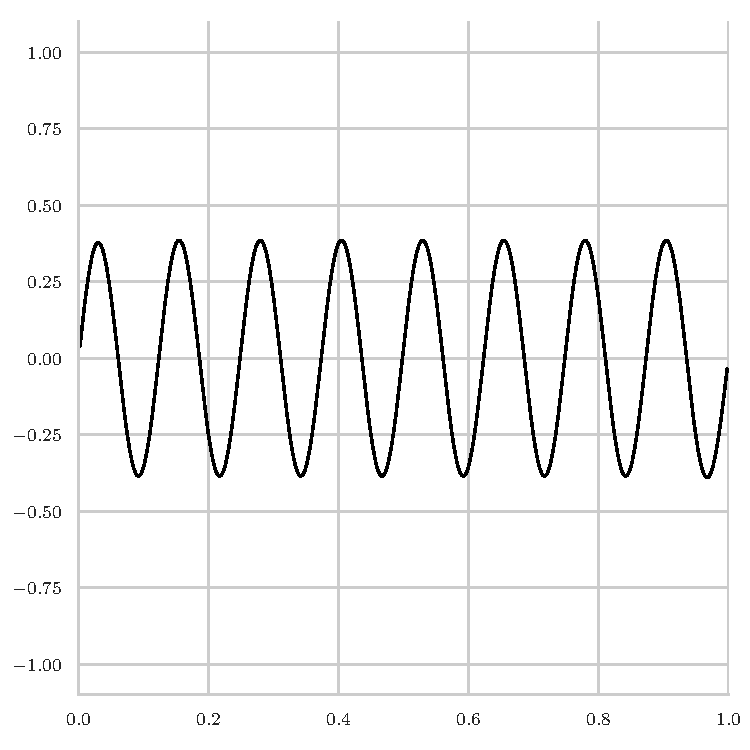
\includegraphics[width=\textwidth]{figures/error_plots//final_error_gauss_seidel_16pi.pdf}
		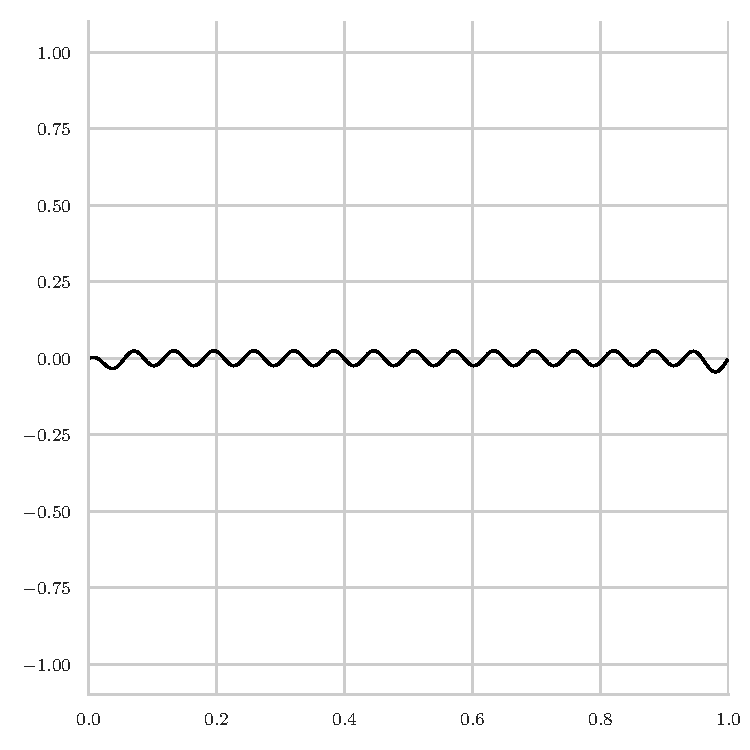
\includegraphics[width=\textwidth]{figures/error_plots//final_error_gauss_seidel_32pi.pdf}
	\caption{Error after applying GS}
	\end{subfigure}
	\caption{Different error components on a one-dimensional grid with step size $h = 2^{-9}$ before and after applying 100 steps of the Jacobi or Gauss-Seidel (GS) method.}
	\label{fig:different-error-components}
\end{figure}
Here, the first column shows the initial error discretized on a grid with step size $h = 2^{-9}$ while the second and third include the remaining error after applying 100 Jacobi and Gauss-Seidel steps, respectively.
Note that the frequency of change increases from top to bottom, whereas the amplitude of the error is always the same.
As can be seen in the second and third column of the first row of Figure~\ref{fig:different-error-components}, the Jacobi and Gauss-Seidel methods do not yield a significant reduction of the low-frequency error components within 100 iterations.
In contrast, in the third row, which shows a highly-oscillating component, the application of 100 steps of the Jacobi method already reduces the initial error to less than one-fifth of its original value.
The same behavior can also be observed for the Gauss-Seidel method, whereby, compared to the Jacobi method, high-frequency error components are reduced even faster.
We can further illustrate the error reduction properties of basic iterative methods by investigating Figure~\ref{fig:combined-error}, which contains a combination of two error components with equal magnitude, one of them with low and the other one with high frequency.
\begin{figure}
	\begin{subfigure}[t]{0.32\textwidth}
	\centering
		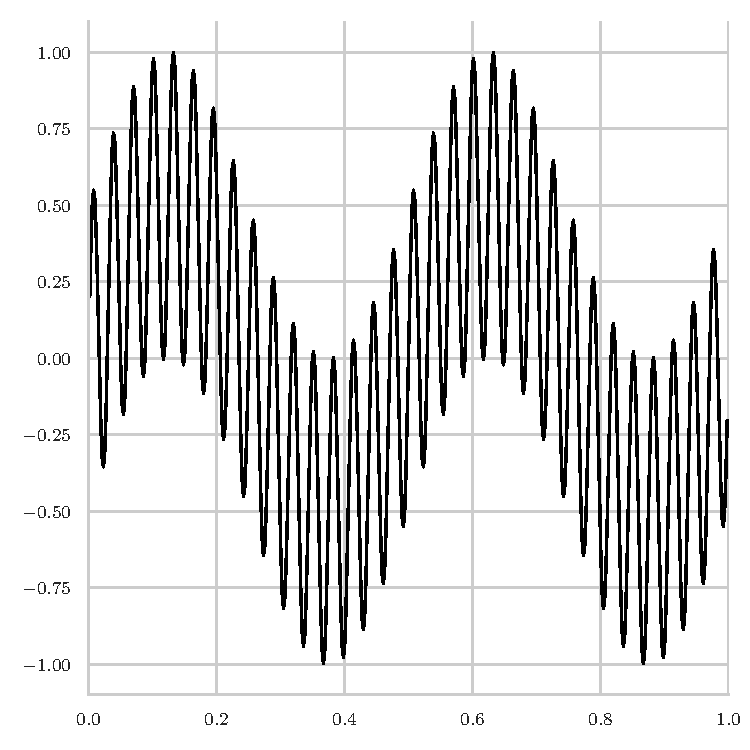
\includegraphics[width=\textwidth]{figures/error_plots//initial_error_jacobi_combined.pdf}
		\caption{Initial error}
\end{subfigure}
\hfill
\begin{subfigure}[t]{0.32\textwidth}
	\centering
		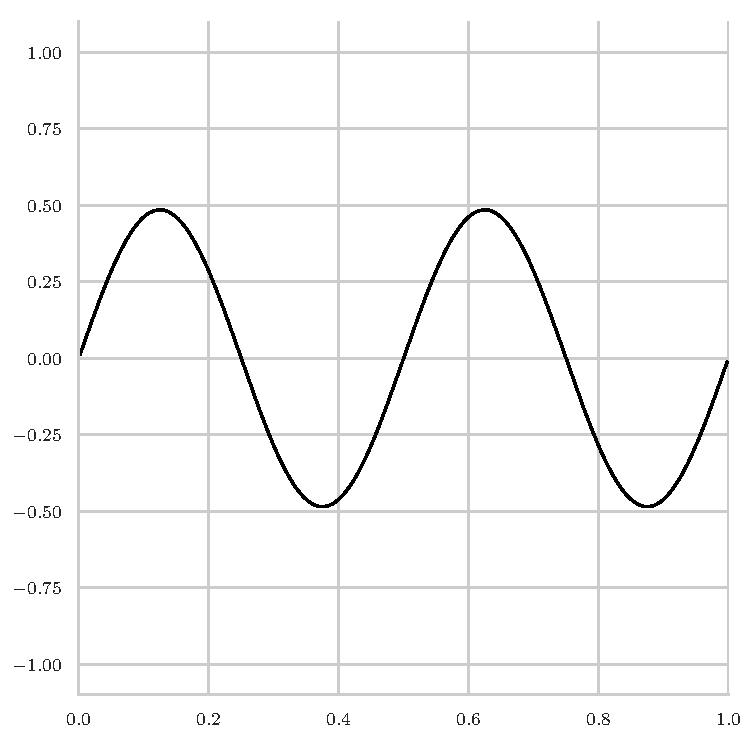
\includegraphics[width=\textwidth]{figures/error_plots//final_error_jacobi_combined.pdf}
		\caption{Error after applying Jacobi}
\end{subfigure}
\begin{subfigure}[t]{0.32\textwidth}
	\centering
	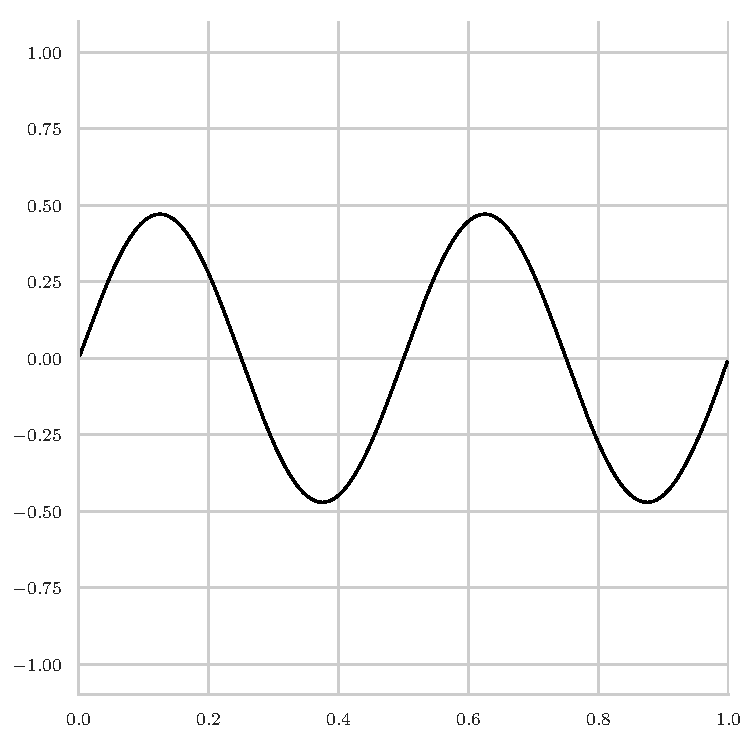
\includegraphics[width=\textwidth]{figures/error_plots//final_error_gauss_seidel_combined.pdf}
	\caption{Error after applying GS}
\end{subfigure}
	\caption{Combination of two error components discretized on a one-dimensional grid with step size $h = 2^{-9}$ before and after applying 100 steps of the Jacobi or Gauss-Seidel (GS) method.}
\label{fig:combined-error}
\end{figure}
Again, the first plot shows the initial error, while the second and third contain the reduced error after 100 iterations of Jacobi and Gauss-Seidel, respectively.
In accordance with our previous observations, the attained improvement achieved with both methods can be almost fully attributed to the reduction of the highly-oscillating component.
Because the remaining error is more smooth than initially, basic iterative methods are often called \emph{smoothers}, and their effectiveness is measured in terms of their capability to reduce the high-frequency components of a given error. 

Now observe what happens if we represent the same low-frequency error component shown in the first row of Figure~\ref{fig:different-error-components} on a grid with larger step size $h = 2^{-6}$ and, thus, a smaller number of grid points.
Because the number of (inner) grid points $n = 1/h - 1$ is inversely proportional to the step size, we call such a grid \emph{coarser}.
The resulting error reduction, again after 100 iterations of each method, is shown in Figure~\ref{fig:low-frequency-error-component-coarse}. 
\begin{figure}
	\begin{subfigure}[t]{0.32\textwidth}
	\centering
	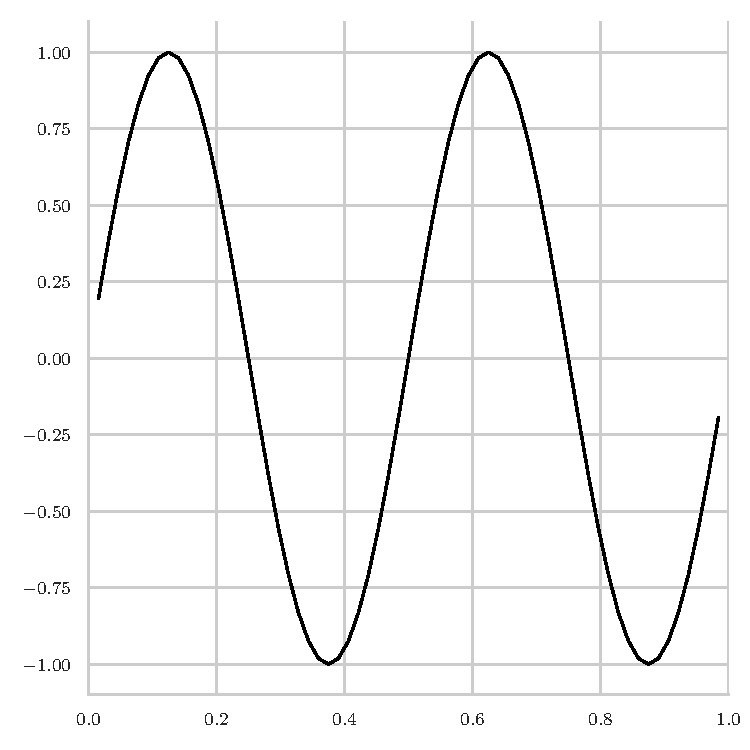
\includegraphics[width=\textwidth]{figures/error_plots//initial_error_jacobi_4pi_coarse.pdf}
	\caption{Initial error}
\end{subfigure}
\hfill
\begin{subfigure}[t]{0.32\textwidth}
	\centering
	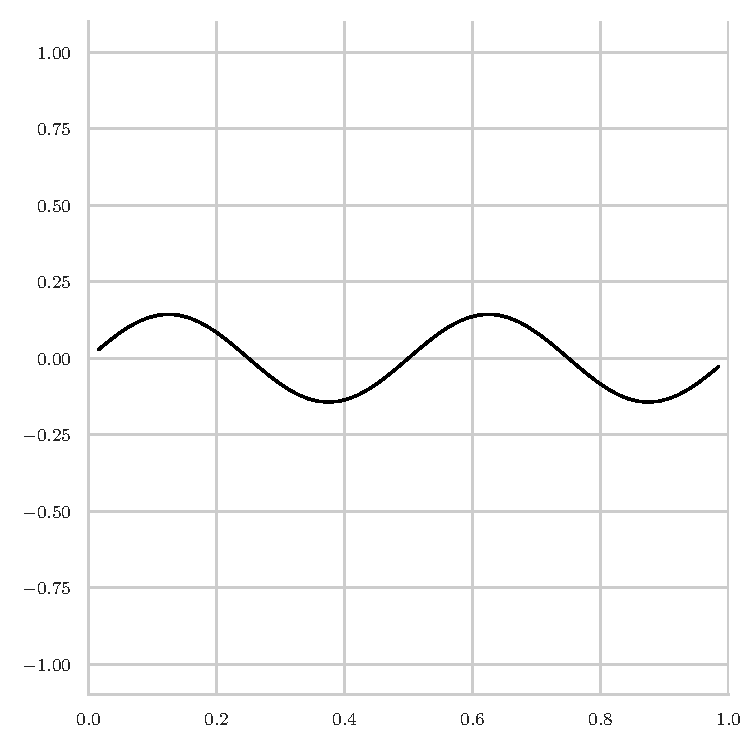
\includegraphics[width=\textwidth]{figures/error_plots//final_error_jacobi_4pi_coarse.pdf}
	\caption{Error after applying Jacobi}
\end{subfigure}
	\hfill
	\begin{subfigure}[t]{0.32\textwidth}
		\centering
		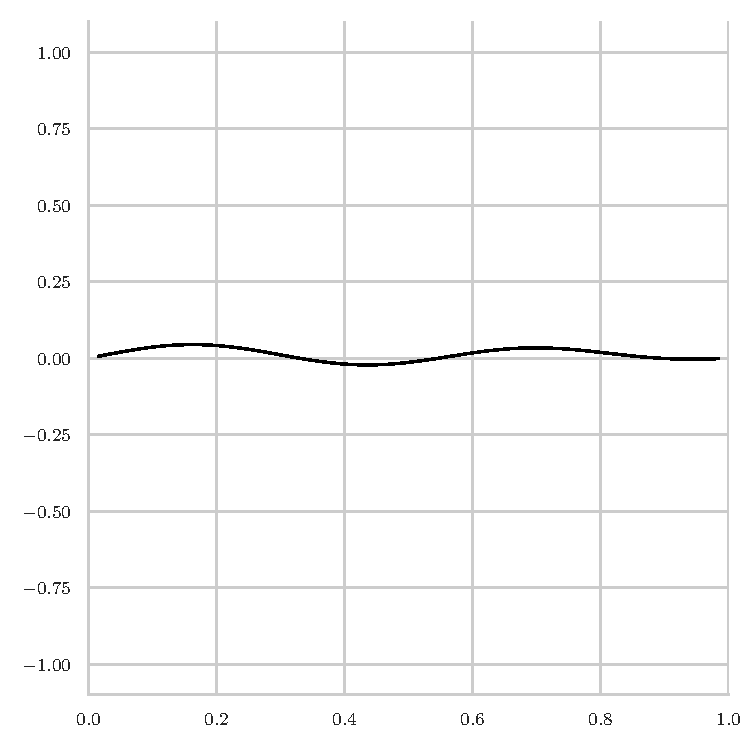
\includegraphics[width=\textwidth]{figures/error_plots//final_error_gauss_seidel_4pi_coarse.pdf}
		\caption{Error after applying GS}
	\end{subfigure}
	\caption{Low-frequency error component discretized on a coarser one-dimensional grid with step size $h = 2^{-6}$ before and after applying 100 steps of the Jacobi or Gauss-Seidel (GS) method.}
	\label{fig:low-frequency-error-component-coarse}
\end{figure}
As it can be seen, the amount of low-frequency error reduction is significantly higher for both methods than on the \emph{finer} grid with a step size of $h = 2^{-9}$.
While smoothers, such as Jacobi and Gauss-Seidel, are only effective in reducing the high-frequency components of a given error, we can overcome this limitation by representing the remaining error on a coarser grid.
Since, on this level, the remaining low-frequency components become more oscillatory, smoothing regains its effectiveness. 
\emph{Multigrid} methods extend this idea by recursively obtaining a coarser representation of the same problem, whose error can then be effectively reduced by employing only a few \emph{smoothing} iterations.
The result is then used to extinguish the remaining error on the next-higher level.
In the following, we introduce the basic components of multigrid methods, i.e., the smoothing, restriction, prolongation, and coarse-grid correction operations.
%Based on this definition, we then develop a formal language for the representation of multigrid solvers.
\subsection{Smoothing}
\label{subsec:smoothing}
One of the central elements of multigrid methods is the utilization of a smoothing procedure for quickly reducing the oscillatory components of a given error.
We have already shown that the Jacobi and Gauss-Seidel method behave in such a way for the considered one-dimensional model problem.
To further improve the smoothing effectiveness of an iterative method, it is often beneficial to introduce an additional relaxation factor $\omega$, which yields the iteration 
\begin{equation}
	\bm{x}^{(k+1)} = \bm{x}^{(k)} + \omega M^{-1}(\bm b - A \bm{x}^{(k)}).
	\label{eq:general-weighted-stationary-iterative-method}
\end{equation}
Again, the weighted Jacobi or Gauss-Seidel method is obtained by replacing the matrix $M$ with the respective term.
\subsubsection{Red-Black Gauss-Seidel}
\label{sec:rb-gs}
While the Gauss-Seidel method often exhibits a superior smoothing property compared to the Jacobi method~\cite{briggs2000multigrid,trottenberg2000multigrid}, each iteration requires solving a lower triangular system of the form
\begin{equation*}
	(D - L) (\bm{x}^{(k+1)} - \bm{x}^{(k)}) = \bm{b} - A \bm{x}^{(k)},
\end{equation*}
with $D - L$ as the lower triangular part of the system matrix $A$.
Since $U = A - (D - L)$, we can rewrite this equation to obtain
\begin{equation}
	(D - L) \bm{x}^{(k+1)} = \bm{b} - U \bm{x}^{(k)},
\end{equation}  
which can then be solved using forward substitution by computing
\begin{equation}
	x_{i}^{(k+1)}={\frac {1}{a_{ii}}}\left(b_{i}-\sum _{j=1}^{i-1}a_{ij}x_{j}^{(k+1)}-\sum _{j=i+1}^{n}a_{ij}x_{j}^{(k)}\right),
	\label{eq:gauss-seidel-element-wise}
\end{equation}
where $x_{i}^{(k)}$ represents the $i$th element of the vector $\bm{x}^{(k)}$.
However, because $x_{i+1}^{(k)}$ depends on $x_{i}^{(k)}$ this computation can only be performed sequentially, which means that the individual components of $\bm{x}^{(k+1)}$ must be computed one after another. 
Modern compute architectures exhibit an ever-increasing degree of parallelism, and hence we must be able to perform all computations in parallel to fully utilize their capabilities.
Now consider the Jacobi method as defined by 
\begin{equation*}
	\bm{x}^{(k+1)} = \bm{x}^{(k)} + D^{-1}(\bm b - A \bm{x}^{(k)}).
\end{equation*}
Similar to the Gauss-Seidel method, we can rewrite this equation to obtain
\begin{equation}
	\bm{x}^{(k+1)} = D^{-1}(\bm b - (A - D)\bm{x}^{(k)}),
\end{equation}
which yields the following element-wise formulation of the Jacobi method:
\begin{equation}
x_{i}^{(k+1)}={\frac {1}{a_{ii}}}\left(b_{i}-\sum _{j\neq i}a_{ij}x_{j}^{(k)}\right).
	\label{eq:jacobi-element-wise}
\end{equation}
In contrast to Equation~\eqref{eq:gauss-seidel-element-wise} the computation of each subsequent element of the vector $\bm{x}^{(k+1)}$ does not depend on any previous one.
Consequently, the computation of each individual element of the new approximate solution $\bm{x}^{(k+1)}$ can be performed completely in parallel.

One possibility to enable a parallel Gauss-Seidel-like computation of the approximate solution $\bm{x}^{(k+1)}$ is to partition the grid points into multiple subsets.
The computation of each subset is then performed in a Jacobi-like fashion using the updated values from other subsets.
A common variant of this approach is the \emph{red-black Gauss-Seidel} (RB-GS) method.
Here, the grid points are assigned to two distinct subsets, where the first represents the red and the second one the black points.
We can define the RB-GS method in the following way:
\begin{equation}
	\begin{split}
		& \bm{x}^{(k+1/2)} = \bm{x}^{(k)} + P_r D^{-1} (\bm{b} - A \bm{x}^{(k)}) \\
		& \bm{x}^{(k+1)} = \bm{x}^{(k+1/2)} + P_b D^{-1} (\bm{b} - A \bm{x}^{(k+1/2)})
	\end{split}
\end{equation}
The entries of the matrices $P_R$ and $P_B$ are then defined as
\begin{equation}
	P_{R,ij} = \begin{cases}
	1 & \text{if} \; i = j \; \text{and} \; i,j \in R \\
	0 & \text{otherwise},  
	\end{cases}
\end{equation}
\begin{equation}
	P_{B,ij} = \begin{cases}
		1 & \text{if} \; i = j \; \text{and} \; i,j \in B \\
		0 & \text{otherwise},
	\end{cases}
\end{equation}
where $R$ and $B$ are the sets of grid indices that correspond to the red and black points, respectively.
For instance, an RB-GS method for the three-point stencil defined in Equation~\eqref{eq:1D-laplace-stencil} can be formulated as
\begin{equation}
\begin{split}
   	& x_{2i}^{(k+1/2)} = \frac {1}{2}\left(h^2 b_{2i} + x_{2i+1}^{(k)} + x_{2i-1}^{(k)}\right) \\
    & x_{2i+1}^{(k+1)} = \frac {1}{2}\left(h^2 b_{2i+1} + x_{2i+2}^{(k+1/2)} + x_{2i}^{(k+1/2)}\right),
\end{split}
\end{equation}
where each grid point with an even index belongs to the red and each one with an odd index to the black points.
Note that the update of each grid point is exclusively based on its neighbors, which have already been updated in the previous step of the method.
By always assigning neighboring points to different partitions, a similar effect can be achieved on any $d$-dimensional grid. 
For instance, a suitable partitioning for the discretized Laplace operator $\Delta_h$ is given by
\begin{equation}
		R = \{ \bm{i} : \bm{i} \in \mathbb{N}^d, \sum_{k=1}^d i_k \; \text{even} \}, \;
		B = \{ \bm{i} : \bm{i} \in \mathbb{N}^d, \sum_{k=1}^d i_k \; \text{odd} \}.
\end{equation}
In many cases, the resulting method has better smoothing properties than the Jacobi method without sacrificing much of its parallelism, as the computations on each partition can be performed concurrently~\cite{trottenberg2000multigrid}.
\subsubsection{Block Smoothing}
\label{subsec:block-smoothing}
So far, we have only discussed smoothers that operate in a pointwise manner.
For instance, in the Jacobi method Equation~\eqref{eq:jacobi-element-wise} is computed for each individual grid point.
The idea of block smoothing is to reorder the original system in such a way, that the same operations can be defined on small subsets of grid points, which are chosen in the form of rectangular blocks of a particular size.
As a consequence, each scalar operation in the original pointwise method is replaced by a matrix or vector operation, whose dimensionality corresponds to the chosen block size.

For example, we can rearrange our original system of the form of Equation~\eqref{eq:general-system-of-linear-equations} in the following way:
\begin{equation}
\underbrace{
\begin{pmatrix}A_{11}&A_{12}&\cdots &A_{1m}\\A_{21}&A_{22}&\cdots &A_{2m}\\\vdots &\vdots &\ddots &\vdots \\A_{m1}&A_{m2}&\cdots &A_{mm}\end{pmatrix}}_{A}
 = 
\underbrace{
\begin{pmatrix}
\bm{x}_1 \\ \bm{x}_2 \\ \vdots \\ \bm{x_m} 
\end{pmatrix}}_{\bm{x}} =
\underbrace{
\begin{pmatrix}
	\bm{b}_1 \\ \bm{b}_2 \\ \vdots \\ \bm{b_m} 
\end{pmatrix}}_{\bm{b}}
\end{equation}
where $m = n / n_b$, if $n_b$ is the size of each block.
A block Jacobi method can then be defined as
\begin{equation}
	\bm{x}_{i}^{(k+1)}=A_{ii}^{-1}\left(\bm{b}_{i}-\sum _{j\neq i}A_{ij}\bm{x}_{j}^{(k)}\right),
	\label{eq:jacobi-block-wise}
\end{equation}
For example, choosing a block size of two for the one-dimensional Laplace equation yields
\begin{equation}
	\begin{pmatrix}
		2 & -1 \\
		-1 & 2
	\end{pmatrix}
	\begin{pmatrix}
		x_{j}^{(k+1)} \\ x_{j+1}^{(k+1)} 
	\end{pmatrix}
= 	-  \begin{pmatrix}
	0 & 0 \\
	-1 & 0
\end{pmatrix} 	
\begin{pmatrix}
x_{j+2}^{(k)} \\ x_{j+3}^{(k)}
\end{pmatrix} -
\begin{pmatrix}
	0 & -1 \\
	0 & 0
\end{pmatrix} 	
\begin{pmatrix}
	x_{j-2}^{(k)} \\ x_{j-1}^{(k)} 
\end{pmatrix},
\end{equation}
where $j = n_b (i - 1) + 1$.
This method can be defined in a similar way using our previously introduced stencil notation
\begin{equation}
\begin{split}
	& \begin{pmatrix}
		\left[0 \quad 2 \quad -1 \right]_{h} \cdot x_{j}^{(k+1)} \\ \left[ -1 \quad 2 \quad 0 \right]_{h} \cdot x_{j+1}^{(k+1)} 
	\end{pmatrix}
	= \\ - & 
	\begin{pmatrix}
		\left[ 0 \right]_{h} \cdot x_{j+2}^{(k)} \\ \left[-1 \quad 0 \quad 0 \right]_{h} \cdot x_{j + 3}^{(k)}
	\end{pmatrix} -
	\begin{pmatrix}
		\left[0 \quad 0 \quad -1 \right]_{h} \cdot x_{j-2}^{(k)} \\ \left[ 0 \right]_{h} \cdot x_{j-1}^{(k)} 
	\end{pmatrix}.
\end{split}
\end{equation}
In both cases, we obtain a system of two linear equations
\begin{equation}
	\begin{pmatrix}
		2 x_{j}^{(k+1)} - x_{j+1}^{(k+1)} \\ 2 x_{j+1}^{(k+1)} - x_{j}^{(k+1)} 
	\end{pmatrix}
	=
	\begin{pmatrix}
		x_{j - 1}^{(k)} \\ x_{j + 2}^{(k)}
	\end{pmatrix}.
\end{equation}
which must be solved for each block, for instance, using a direct solver such as Gaussian elimination.
As in the pointwise Jacobi method, each block can be solved independently and, therefore, operations on different blocks can be performed in parallel. 
Considering the fact that a direct solver in general require $\mathcal{O}(n_b^3)$ operations to solve each block, the overall computational cost of applying a block smoother can be estimated with $\mathcal{O}(n_b^3 \frac{n}{n_b}) = \mathcal{O}(n_b^2 n)$.
Note that choosing $n_b = n$ means that we treat the whole matrix $A$ as a single block and, therefore, solve the original system using Gaussian elimination.
In contrast, the choice of $n_b = 1$ corresponds to the pointwise Jacobi method, which, for a constant stencil, can be computed with a constant number of operations per grid point.
While we here only provide a brief introduction to block smoothers, it must be mentioned that it is also possible to define block variants for other smoothers, such as the Gauss-Seidel and red-black Gauss-Seidel method.
Finally, alternatively, it is also possible to define overlapping block smoothers, which means that multiple blocks contain the same grid point as an unknown~\cite{trottenberg2000multigrid}.

\subsection{The Coarse-Grid Correction Scheme}
The core idea behind multigrid methods is to reduce the oscillatory components of an error by obtaining an approximation of the same problem on a coarser grid.
As we have illustrated in Figure~\ref{fig:low-frequency-error-component-coarse} these components can then be reduced quickly using the same smoothing techniques employed on the fine grid.
Before we can define this approach algorithmically, note that our original system
\begin{equation}
	A_h \bm{x}_h = \bm{b}_h
\end{equation}
is equivalent to the error equation
\begin{equation}
	A_h \left(\bm{x}_h - \bm {x}^{(0)}_h\right) = \bm{b}_h - A_h \bm{x}^{(0)}_h
\end{equation}
with the arbitrary-chosen initial guess $\bm{x}^{(0)}_h$.
The subscripts $A_h$ and $\bm{x}_h$ indicate a discretization with step size $\bm{h}$.
Therefore, each entry of the vector $\bm{x}_h$ represents a grid function value $u_h(\bm{i} \cdot \bm{h})$ at the respective position within the grid.
We can further introduce the error $\bm{e}_h = \bm{x}_h - \bm {x}^{(0)}_h$ to obtain the equation
\begin{equation}
	A \bm{e} = \bm{b} - A \bm{x}^{(0)}.
	\label{eq:linear-system-error-equation}
\end{equation}
Based on the solution $\bm{e}_h$ of this system, which depends on the initial solution $\bm{x}^{(0)}_h$, we can, again, obtain the solution of the original system by computing
\begin{equation}
	\bm{x}_h = \bm{x}^{(0)}_h + \bm{e}_h.
\end{equation}
Now, assume there exists both a prolongation and restriction operator, $I_h^{2h}$ and $I_{2h}^h$, that enables us to compute an approximation for a given variable $\bm{x}_h$ on a coarser and finer grid, respectively, such that
\begin{equation}
	\bm{x}_{2h} \approx I_h^{2h} \bm{x}_{h}, \;
	\bm{x}_{h} \approx I_{2h}^{h} \bm{x}_{2h}. 
\end{equation}
In general, this approximation can obviously never be exact.
However, we have already observed that if a certain error exclusively consists of smooth components, we can approximate them on a coarser grid without a significant loss of accuracy.
This is illustrated in Figure~\ref{fig:error-on-multiple-levels}, which shows the discretization of two error components with different frequencies on one-dimensional uniform grids with decreasing step size.
Here, the first error component, which possesses a higher frequency, can not be accurately represented on the coarsest grid with step size $h = 2^{-5}$.
In contrast, the course of the second error component, which is relatively smooth, is still clearly visible on the same grid. 
\begin{figure}
	\begin{subfigure}[b]{0.32\textwidth}
		\centering
		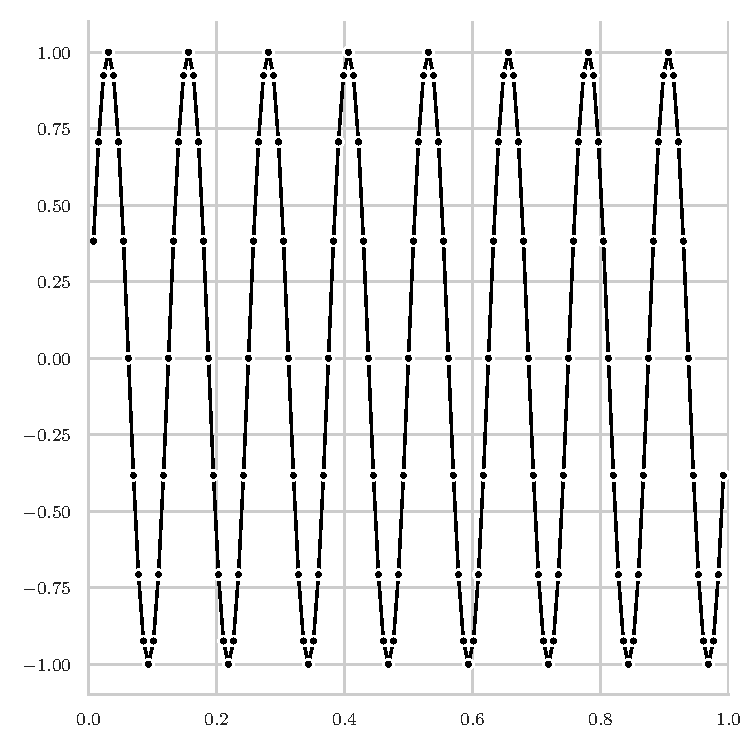
\includegraphics[width=\textwidth]{figures/error_plots//initial_error_16pi_level7.pdf}
	\end{subfigure}
	\hfill
	\begin{subfigure}[b]{0.32\textwidth}
		\centering
		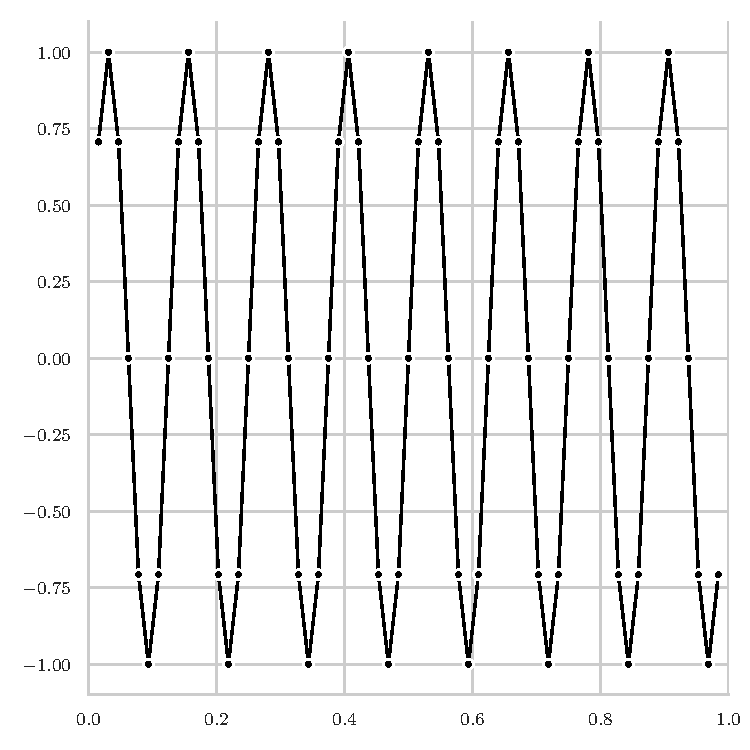
\includegraphics[width=\textwidth]{figures/error_plots//initial_error_16pi_level6.pdf}
	\end{subfigure}
	\hfill
	\begin{subfigure}[b]{0.32\textwidth}
		\centering
		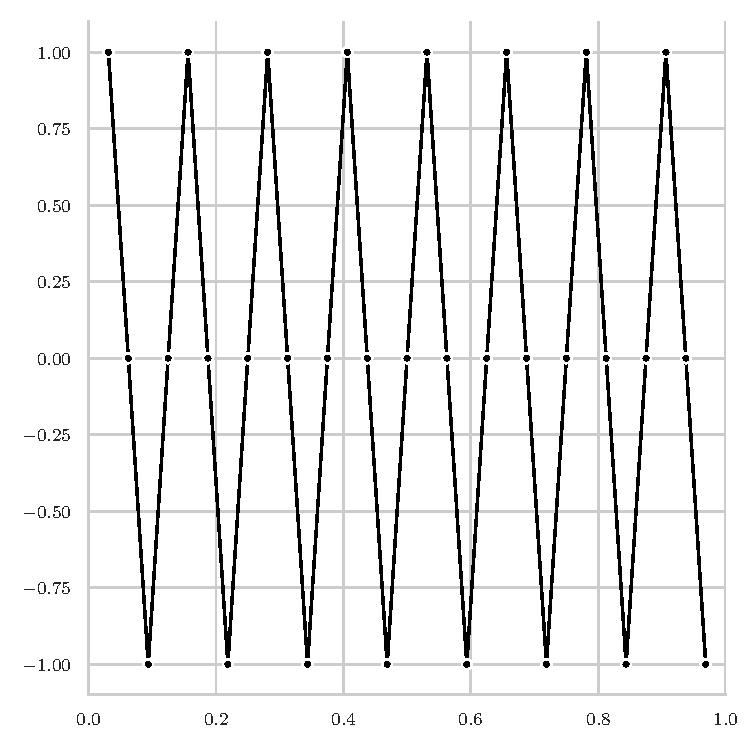
\includegraphics[width=\textwidth]{figures/error_plots//initial_error_16pi_level5.pdf}
	\end{subfigure}
		\begin{subfigure}[b]{0.32\textwidth}
		\centering
		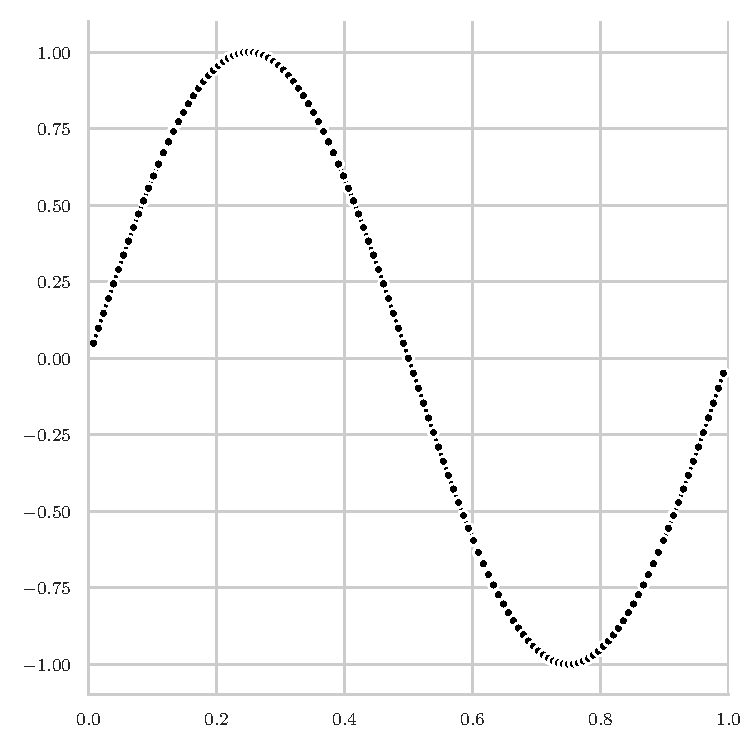
\includegraphics[width=\textwidth]{figures/error_plots//initial_error_2pi_level7.pdf}
		\caption{$h = 2^{-7}$}
	\end{subfigure}
	\hfill
	\begin{subfigure}[b]{0.32\textwidth}
		\centering
		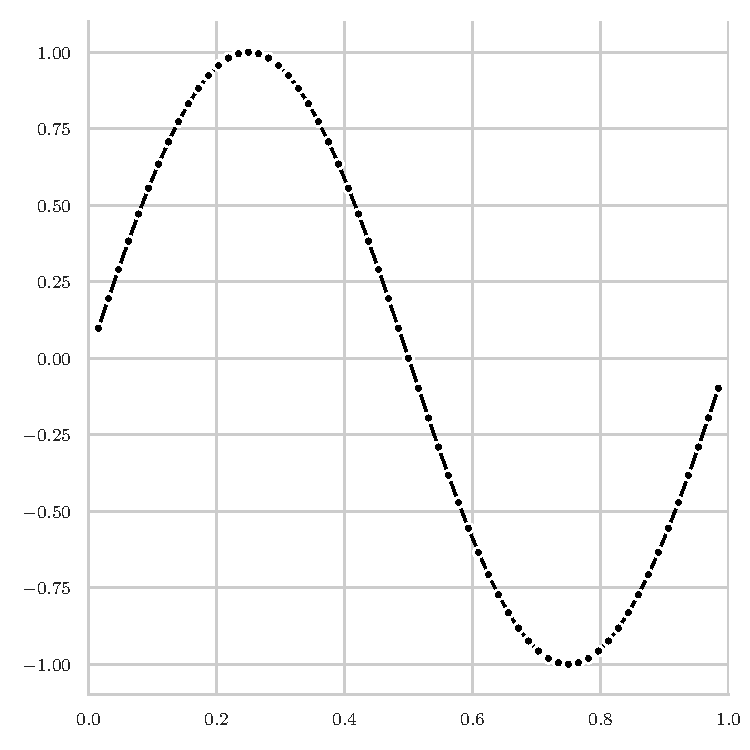
\includegraphics[width=\textwidth]{figures/error_plots//initial_error_2pi_level6.pdf}
		\caption{$h = 2^{-6}$}
	\end{subfigure}
	\hfill
	\begin{subfigure}[b]{0.32\textwidth}
		\centering
		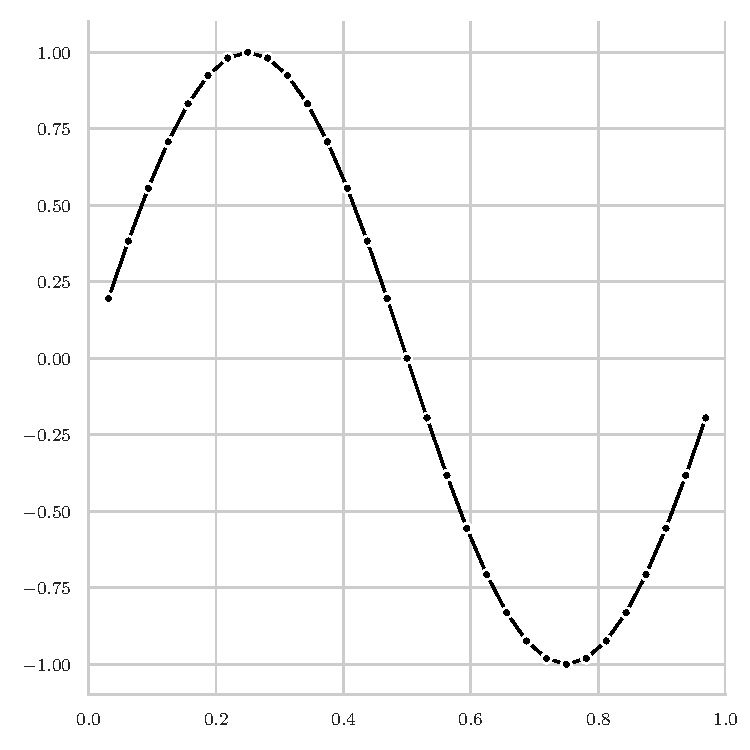
\includegraphics[width=\textwidth]{figures/error_plots//initial_error_2pi_level5.pdf}
		\caption{$h = 2^{-5}$}
	\end{subfigure}
	\caption{Oscillatory and smooth error components discretized on a hierarchy of grids with decreasing step size.}
	\label{fig:error-on-multiple-levels}
\end{figure}
Assuming that the error $\bm{e}_{2h}$ on the coarse grid consists exclusively of smooth components and, hence, $\bm{e}_{h} \approx I_{2h}^{h} \bm{e}_{2h}$, we can define the coarse grid correction 
\begin{equation}
	\bm{x}^{k+1}_h = \bm{x}^{k}_h + I_{2h}^h \bm{e}_{2h}.
\end{equation} 
Now the question remains to be answered how we can compute an approximation for the error $\bm{e}_{2h}$ on the coarse grid.
As we have pointed out above, Equation~\eqref{eq:linear-system-error-equation} is equivalent to the original system.
We can, therefore, can apply our previously defined inter-grid transfer operators to define the error equation on a coarser grid with step size $2\bm{h}$
\begin{equation}
	\underbrace{I_{h}^{2h} A_h I_{2h}^h}_{A_{2h}} \bm{e}_{2h} = I_{h}^{2h} \left(\bm{b}_h - A_h \bm{x}^{(0)}_h\right).
	\label{eq:coarse-grid-error-equation}
\end{equation}
Note that we have again made use of the fact that in case $\bm{e}_{2h}$ is smooth, $\bm{e}_{h} \approx I_{2h}^{h} \bm{e}_{2h}$ is a reasonably accurate approximation.
Note that in Equation~\eqref{eq:coarse-grid-error-equation} the coarse operator $A_{2h}$ is directly obtained from the original operator $A_{2h}$, which is called \emph{Galerkin coarsening}.
However, in cases where the operator $A_h$ can be directly discretized on a coarser grid with step size $2\bm{h}$, it is often also possible to use the resulting operator $A_{2h}$ instead.
By bringing all these components together, we can formulate the two-level-method shown in Algorithm~\ref{alg:two-grid-method}.
\begin{algorithm}
	\caption{Two-Grid Method}
	\label{alg:two-grid-method}
	\begin{algorithmic}
		\State{Relax on $A_h \bm{x}_h = \bm{b}_h$ to obtain an approximation $\tilde{\bm{x}}_h$}
		\State{Compute the residual $\bm{r}_h = \bm{b}_h - A_h \tilde{\bm {x}}_h$}
		\State{\hskip1em Obtain $A_{2h}$ through Galerkin coarsening or rediscretization}
		\State{\hskip1em Restrict the residual $\bm{b}_{2h} = I_h^{2h} \bm{r}_h$}
		\State{\hskip1em Solve $A_{2h} \bm{x}_{2h} = \bm{b}_{2h}$ for $\bm{x}_{2h}$}
		\State{Perform the correction $\tilde{\bm{x}}_h = \tilde{\bm{x}}_h + I_{2h}^h \bm{x}_{2h}$}
		\State{Relax again $A_h \bm{x}_h = \bm{b}_h$ with an initial guess of $\tilde{\bm{x}}_h$}
	\end{algorithmic}
\end{algorithm}
Note that while on the coarse grid we are actually solving the error equation, it has been redefined as $A_{2h} \bm{x}_{2h} = \bm{b}_{2h}$.
Based on this notation, we could similarly define a two-level method starting from a grid with step size $2\bm{h}$.
However, to put this approach into practice, we need to choose an initial guess for the error equation on this level.
For this purpose, note that one step of smoothing applied to Equation~\eqref{eq:coarse-grid-error-equation} with an initial guess of zero corresponds to
\begin{equation}
	\bm{e}_{2h}^{(1)} = M_{2h}^{-1} I_{h}^{2h} \left(\bm{b}_h - A_h \bm{x}^{(0)}_h\right).
	\label{eq:initial-coarse-grid-relaxation}
\end{equation}
Since the error $\bm{e}_{2h}^{(k+1)}$ in step $k+1$ is defined as
\begin{equation*}
	\bm{e}_{2h}^{(k+1)} = \bm{x}_{2h}^{(k+1)} - \bm{x}_{2h}^{(k)},
\end{equation*}
and assuming that $\bm{x}_{h}^{(0)}$ is smooth, we can choose $\bm{x}_{2h}^{(0)} = I_{2h}^{h} \bm{x}_{h}^{(0)}$ and, hence, obtain the iteration
\begin{equation}
	\bm{x}_{2h}^{(1)} = I_{h}^{2h} \bm{x}_{h}^{(0)} + M_{2h}^{-1} ( I_{h}^{2h} \bm{b}_h - \underbrace{I_{h}^{2h} A_h I_{2h}^{h}}_{A_{2h}} I_{h}^{2h} \bm{x}_{h}^{(0)} ).
\end{equation}
Performing one smoothing step with an initial guess of zero on the coarse-grid error equation, therefore, corresponds to one smoothing step applied to the equation
\begin{equation}
	I_{h}^{2h} A_h I_{2h}^h \bm{x}_{2h} = I_{h}^{2h} \bm{b}_h,
\end{equation}
with an initial guess of $\bm{x}_{2h}^{(0)} = I_{h}^{2h} \bm{x}_{h}^{(0)}$.
Because smoothing aims to remove the remaining oscillatory components of the error that have been transferred from the fine grid, applying it in the form of Equation~\eqref{eq:initial-coarse-grid-relaxation} precisely serves this purpose.

\subsection{Restriction and Prolongation}
\label{subsec:restriction-and-prolongation}
%TODO fix stencil notation in this section
Before we can define an actual multigrid method, which recursively applies the techniques introduced here to a hierarchy of discretizations consisting of more than two levels, we need to define suitable inter-grid operators, $I_{2h}^{h}$ and $I_{h}^{2h}$.
Here, the restriction operator $I_{2h}^{h}$ should yield an accurate approximation of the current residual on a coarser grid, while the goal of the prolongation operator $I_{h}^{2h}$ is to transfer the computed solution of the error equation back to a finer grid.
In both cases, we are, first and foremost, interested in preserving the low-frequency components, as the remaining ones will be quickly reduced by smoothing.
In general, the implementation of these operators depends on the chosen method of discretization. 
Since, as mentioned in Section~\ref{sec:discretization}, this work focuses on the discretizations of PDEs on regular grids, we do not consider inter-grid operators defined on other grid types, such as unstructured grids.
For a detailed treatment of these cases, the reader is referred to~\cite{trottenberg2000multigrid,ruge1987algebraic,stuben2001introduction}.
As a first step towards defining a suitable restriction operator, note that on a regular grid, the set of coarse-grid points is always contained in the set of fine-grid points.
Therefore, the easiest way to define such an operator is to simply carry over the values present at the respective points of the fine grid over to the coarse grid, which leads to the so-called \emph{injection} restriction operator.
While this approach can lead to a functioning multigrid method in case the residual is sufficiently smooth, it neglects the information contained within all fine grid points that do not coincide with a coarse grid point.
In most cases, it is beneficial to incorporate this information into the coarse grid by computing a weighted average over all neighboring fine grid points.
This idea leads to the so-called \emph{full-weighting} and \emph{half-weighting} restriction operators.
Using our previously defined stencil notation, the one-dimensional full-weighting restriction operator is given by
\begin{equation}
	I_{h}^{2 h} = \frac{1}{4}\{((-1), 1), ((0), 2), ((1), 1)\}_{h_x}^{2h}
\end{equation} 
or equivalently using the matrix notation
\begin{equation}
	I_{h}^{2h} =  \frac{1}{4} \begin{bmatrix}
			1 & 2 & 1
		\end{bmatrix}_{h_x}^{2h}.
	\label{eq:full-weighting-restriction}
\end{equation} 
If we treat Equation~\eqref{eq:full-weighting-restriction} as a row vector, we can define the two- and three-dimensional full-weighting restriction operator as a tensor product with the corresponding column vector, such that
\begin{equation}
	I^{2h_x, 2h_y}_{h_x, h_y} = \frac{1}{4} \begin{bmatrix}
		1 \\ 2 \\ 1
	\end{bmatrix}_{h_y}^{2h_y} \otimes \frac{1}{4} \begin{bmatrix}
		1 & 2 & 1
	\end{bmatrix}_{h_x}^{2h_x} =
\frac{1}{16} 
\begin{bmatrix}
	1 & 2 & 1 \\
	2 & 4 & 2 \\
	1 & 2 & 1
\end{bmatrix}^{2h_x, 2h_y}_{h_x, h_y},
\end{equation} 
\begin{equation}
\begin{split}
	& I^{2h_x, 2h_y, 2h_z}_{h_x, h_y, h_z} = \frac{1}{4} \begin{bmatrix}
		1 & 2 & 1
	\end{bmatrix}_{h_z}^{2h_z} \otimes 
	\frac{1}{16} 
	\begin{bmatrix}
		1 & 2 & 1 \\
		2 & 4 & 2 \\
		1 & 2 & 1
	\end{bmatrix}^{2h_x, 2h_y}_{h_x, h_y} \\
& = \frac{1}{64} \begin{bmatrix}
\begin{bmatrix}
	1 & 2 & 1 \\
	2 & 4 & 2 \\
	1 & 2 & 1
\end{bmatrix} &	\begin{bmatrix}
2 & 4 & 2 \\
4 & 8 & 4 \\
2 & 4 & 2
\end{bmatrix} &
\begin{bmatrix}
	1 & 2 & 1 \\
	2 & 4 & 2 \\
	1 & 2 & 1
\end{bmatrix}
\end{bmatrix}^{2h_x, 2h_y, 2h_z}_{h_x, h_y, h_z}.
\end{split}
\end{equation}
A second restriction operator based on the idea of averaging neighboring fine grid points is the half-weighting restriction operator, whose two- and three-dimensional versions can be defined as
\begin{equation}
	I^{2h_x,2h_y}_{h_x, h_y} = \frac{1}{8}
	\begin{bmatrix}
		0 & 1 & 0 \\
		1 & 4 & 1 \\
		0 & 1 & 0
	\end{bmatrix}^{2h_x}_{h_x},
\end{equation} 
\begin{equation}
\begin{split}
	& I^{2h_x, 2h_y, 2h_z}_{h_x, h_y, h_z} = 
\frac{1}{4} \begin{bmatrix}
	1 & 2 & 1
\end{bmatrix}_{h_z}^{2h_z}
\otimes 
\frac{1}{8}
	\begin{bmatrix}
	0 & 1 & 0 \\
	1 & 4 & 1 \\
	0 & 1 & 0 
\end{bmatrix}^{2h_x,2h_y}_{h_x, h_y} \\
& =
\frac{1}{32} \begin{bmatrix}
	\begin{bmatrix}
		& 1 &  \\
		1 & 4 & 1 \\
		& 1 & 
	\end{bmatrix}
 &		\begin{bmatrix}
 	& 2 &  \\
 	2 & 6 & 2 \\
 	& 2 & 
 \end{bmatrix} &
	\begin{bmatrix}
	& 1 &  \\
	1 & 4 & 1 \\
	& 1 & 
\end{bmatrix}
\end{bmatrix}^{2h_x, 2h_y, 2h_z}_{h_x, h_y, h_z}
\end{split}
\end{equation} 
Note that in contrast to our original definition of the stencil application in Equation~\eqref{eq:stencil-application}, which applies the stencil to each point on the current grid, the restriction stencils presented here only have to be applied to each point on the fine grid that coincides with a coarse-grid point.
We can therefore replace it with the following slightly adapted definition of stencil application
\begin{equation}
	\begin{split}
		& I_{h}^{2h} \cdot u_h(\bm{x}) = \sum_{k=1}^m b_k u_h({\bm x + \bm{a}_k} \circ \bm{h}) \quad 
		\text{with} \; \bm{x} \in G_{2h}, m \in \mathbb{N} \\ & (\bm{a}_k, b_k) \in I_{h}^{2h} \; \forall \, k \in \{ 1, 2, \dots, m \}
	\end{split}
	\label{eq:stencil-restriction-application}
\end{equation}
where $u_h(\bm{x})$ with $\bm{x} \in G_{2h}$ represents an arbitrary point on the fine grid for which there exists a unique coarse-grid point defined at the same spatial position within the computational domain.
Note that this is an immediate consequence of the fact that we have defined the set of coarse-grid points as a subset of the fine-grid points.

On the other hand, for prolongation, our goal is to define an operator that transfers an approximation of the error computed on a certain discretization level to a grid of higher resolution.
We, therefore, must be able to restore a higher number of grid points based on the given values on the coarse grid, which can be regarded as a distribution process.
The application of this operator to a given coarse-grid point $u_{2h}(\bm{x})$ with $\bm{x} \in G_{2h} \supset G_h$ can be defined as
\begin{equation}
	I_{h}^{2h} \cdot u_{2h}(\bm{x}) \rightarrow
	\begin{cases}
		& \forall \, (\bm{a}_k, b_k) \in I_{2h}^{h} \; \text{with} \; k \in \{ 1, 2, \dots, m \} \; \wedge \; \bm{x} \in G_{2h} : \\
		& u_{h}(\bm{x} + \bm{a}_k \circ \bm{h}) = u_{h}(\bm{x} + \bm{a}_k \circ \bm{h}) + b_k u_{2h}(\bm{x}) 
	\end{cases},
	\label{eq:stencil-prolongation application}
\end{equation}
whereby we assume that initially $\forall u_h(\bm{x}) \; \text{with} \; \bm{x} \in \mathcal G_h : u_h(\bm{x}) = 0$.
A common choice for one-dimensional prolongation is the linear interpolation operator~\cite{trottenberg2000multigrid}, which can be defined as
\begin{equation}
	I_{h_x}^{2h} =  \frac{1}{2} \begin{bmatrix}
		1 & 2 & 1
	\end{bmatrix}_{h}^{2h}.
	\label{eq:linear-interpolation}
\end{equation}
Similar to full-weighting restriction, we can derive two- and three-dimensional versions of this operator as tensor products of the form
\begin{equation}
	I_{h_x, h_y}^{2h_x, 2h_y} = \frac{1}{2} \begin{bmatrix}
		1 \\ 2 \\ 1
	\end{bmatrix}_{h_y}^{2h_y} \otimes \frac{1}{2} \begin{bmatrix}
		1 & 2 & 1
	\end{bmatrix}_{h_x}^{2h_x} =
	\frac{1}{4} 
	\begin{bmatrix}
		1 & 2 & 1 \\
		2 & 4 & 2 \\
		1 & 2 & 1
	\end{bmatrix}_{h_x, h_y}^{2h_x, 2h_y},
\end{equation}
\begin{equation}
	\begin{split}
		I_{h_x, h_y, h_z}^{2h_x, 2h_y, 2h_z} = & \frac{1}{2} \begin{bmatrix}
			1 & 2 & 1
		\end{bmatrix}_{2h}^{h} \otimes 
		\frac{1}{4} 
		\begin{bmatrix}
			1 & 2 & 1 \\
			2 & 4 & 2 \\
			1 & 2 & 1
		\end{bmatrix}_{2h}^{h} \\
		= & \frac{1}{8} \begin{bmatrix}
			\begin{bmatrix}
				1 & 2 & 1 \\
				2 & 4 & 2 \\
				1 & 2 & 1
			\end{bmatrix}&	\begin{bmatrix}
				2 & 4 & 2 \\
				4 & 8 & 4 \\
				2 & 4 & 2
			\end{bmatrix} &
			\begin{bmatrix}
				1 & 2 & 1 \\
				2 & 4 & 2 \\
				1 & 2 & 1
			\end{bmatrix}
		\end{bmatrix}_{2h}^{h} .
	\end{split}
\end{equation}
Finally, we want to emphasize again that while the prolongation and restriction operators presented here represent a common choice for regular grids with uniform step sizes, for instance, the discretization of PDEs with varying coefficients often necessitates the use of more complex operators, such as~\cite{dendy1982black}.

\subsection{The Multigrid Cycle}\label{sec:multigrid-cycles}
By putting this all together, we can now implement a recursive version of Algorithm~\ref{alg:two-grid-method}, that allows us to perform an arbitrary number of coarsening steps until the resulting system of linear equation is small enough to be solved precisely.
The resulting implementation of a \emph{multigrid cycle} in the form of the function \textsc{mg-cycle} is shown in Algorithm~\ref{alg:multigrid-cycle}.
\begin{algorithm}[h]
	\caption{Multigrid Cycle}
	\label{alg:multigrid-cycle}
	\begin{algorithmic}
		\Function{mg-cycle}{$\tilde{\bm{x}}_h$, $A_h$, $\bm{b}_h$, $l$, $\gamma$, $\nu_1$, $\nu_2$, $\omega$}
		\For{$i = 1, \dots, \nu_1$}
		\State{$\tilde{\bm{x}}_h = \tilde{\bm{x}}_h + \omega M_h^{-1} \left( \bm{b}_h - A_h \tilde{\bm{x}}_h \right)$ where $A_h = M_h + N_h$}
		\EndFor
		\State{$\bm{r}_h = \bm{b}_h - A_h \tilde{\bm {x}}_h$}
		\State{$\bm{b}_{2h} = I_h^{2h} \bm{r}_h$}
		\If{$l = 0$}
		\State{ Solve $A_{2h} \bm{x}_{2h} = \bm{b}_{2h}$ for $\bm{x}_{2h}$}
		\Else
		\State{$\tilde{\bm{x}}_{2h} = \bm{0}_{2h}$}
		\For{$i = 1, \dots, \gamma$}
		\State{$\tilde{\bm{x}}_{2h} =  \textsc{mg-cycle}(\tilde{\bm{x}}_{2h}, A_{2h}, \bm{b}_{2h}, l-1, \gamma, \nu_1, \nu_2)$}
		\EndFor
		\EndIf
		\State{$\tilde{\bm{x}}_h = \tilde{\bm{x}}_h + I_{2h}^h \tilde{\bm{x}}_{2h}$}
		\For{$i = 1, \dots, \nu_2$}
		\State{$\tilde{\bm{x}}_h = \tilde{\bm{x}}_h + \omega M_h^{-1} \left( \bm{b}_h - A_h \tilde{\bm{x}}_h \right)$ where $A_h = M_h + N_h$}
		\EndFor
		\State \Return{$\tilde{\bm{x}}_h$}
		\EndFunction
	\end{algorithmic}
\end{algorithm}
Note that this function has a number of additional parameters compared to our original two-grid method.
First of all, $l$ defines the number of recursive coarsening steps until the respective system of linear equations is solved directly.
Furthermore, since, in certain cases, a single recursive application of this function is not sufficient to obtain a reasonably accurate approximation on the coarse grid, additional coarse-grid correction steps can be performed, as controlled by the parameter $\gamma$.
Finally, the parameters $\nu_1$ and $\nu_2$ specify the number of smoothing steps before and after the coarse grid correction is performed, respectively.
Note that when performing multiple sweeps of smoothing or coarse grid correction, the initial guess is, as usual, replaced by the approximation obtained in the previous step.
While in principle, the parameters of \textsc{mg-cycle} can be freely chosen, one usually classifies multigrid cycles according to the choice of $\gamma$, as each value yields a distinct computational pattern.
For instance, choosing $\gamma = 1$ means that only a single recursive descent is performed on each discretization level.
Figure~\ref{fig:three-grid-cycles} and~\ref{fig:four-grid-cycles} illustrate the algorithmic structure resulting from different values of $\gamma$ on a hierarchy of three and four grids, respectively.
\begin{figure}
\centering
	\captionsetup{justification=centering}
   \begin{subfigure}{0.1\textwidth}
		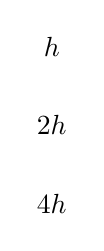
\begin{tikzpicture}
			\node   (h) at (-0.75, 4){$h$};
			\node   (2h) at (-0.75, 3){$2h$};
			\node   (4h) at (-0.75, 2){$4h$};
		\end{tikzpicture}
		\subcaption*{}
	\end{subfigure}
	\begin{subfigure}{0.22\textwidth}
		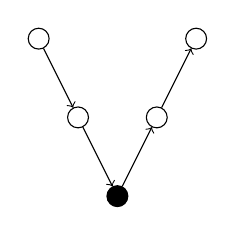
\begin{tikzpicture}
			\node	(a) at (0,4) [draw, circle,scale=0.8] {};
			\node	(b) at (0.5,3) [draw, circle,scale=0.8] {};
			\node	(c) at (1,2) [draw, circle,,fill=black,scale=0.8] {};
			\node	(d) at (1.5,3) [draw, circle,scale=0.8] {};
			\node	(e) at (2,4) [draw, circle, scale=0.8] {};
			
			\draw 
			(a) edge[->] (b) 
			(b) edge[->] (c)
			(c) edge[->] (d)
			(d) edge[->] (e)   
			;
		\end{tikzpicture}
		\subcaption*{$\gamma = 1$}
	\end{subfigure}
	\begin{subfigure}{0.32\textwidth}
		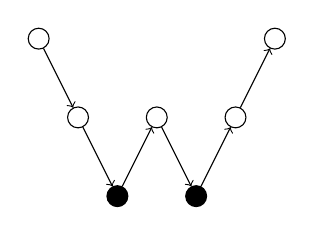
\begin{tikzpicture}
			\node	(a) at (0,4) [draw, circle,scale=0.8] {};
			\node	(b) at (0.5,3) [draw, circle,scale=0.8] {};
			\node	(c) at (1,2) [draw, circle,fill=black,scale=0.8] {};
			\node	(d) at (1.5,3) [draw, circle,scale=0.8] {};
			\node	(e) at (2,2) [draw, circle, fill=black, scale=0.8] {};
			\node	(f) at (2.5,3) [draw, circle, scale=0.8] {};
			\node	(g) at (3,4) [draw, circle, scale=0.8] {};
			
			\draw 
			(a) edge[->] (b) 
			(b) edge[->] (c)
			(c) edge[->] (d)
			(d) edge[->] (e)   
			(e) edge[->] (f)
			(f) edge[->] (g)
			;
		\end{tikzpicture}
		\subcaption*{$\gamma = 2$}
	\end{subfigure}
	\begin{subfigure}{0.32\textwidth}
		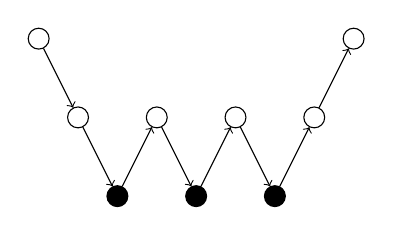
\begin{tikzpicture}
			\node	(a) at (0,4) [draw, circle,scale=0.8] {};
			\node	(b) at (0.5,3) [draw, circle,scale=0.8] {};
			\node	(c) at (1,2) [draw, circle,fill=black,scale=0.8] {};
			\node	(d) at (1.5,3) [draw, circle,scale=0.8] {};
			\node	(e) at (2,2) [draw, circle, fill=black, scale=0.8] {};
			\node	(f) at (2.5,3) [draw, circle, scale=0.8] {};
			\node	(g) at (3,2) [draw, circle, fill=black,scale=0.8] {};
			\node	(h) at (3.5,3) [draw, circle, scale=0.8] {};	
			\node	(i) at (4,4) [draw, circle, scale=0.8] {};	
			\draw 
			(a) edge[->] (b) 
			(b) edge[->] (c)
			(c) edge[->] (d)
			(d) edge[->] (e)   
			(e) edge[->] (f)
			(f) edge[->] (g)
			(g) edge[->] (h)
			(h) edge[->] (i)
			;
		\end{tikzpicture}
		\subcaption*{$\gamma = 3$}
	\end{subfigure}
	\caption{Three-grid cycles ($l = 2$).}
	\label{fig:three-grid-cycles}
\end{figure}
\begin{figure}
	\captionsetup{justification=centering}
	\begin{subfigure}{0.1\textwidth}
		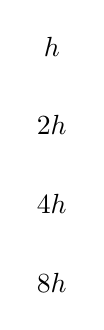
\begin{tikzpicture}
			\node   (h) at (-0.75, 4){$h$};
			\node   (2h) at (-0.75, 3){$2h$};
			\node   (4h) at (-0.75, 2){$4h$};
			\node   (8h) at (-0.75, 1){$8h$};
		\end{tikzpicture}
		\subcaption*{}
	\end{subfigure}
	\begin{subfigure}{0.3\textwidth}
		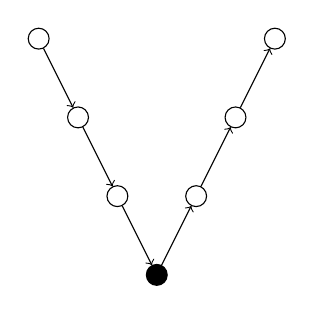
\begin{tikzpicture}
			\node	(a) at (0,4) [draw, circle,scale=0.8] {};
			\node	(b) at (0.5,3) [draw, circle,scale=0.8] {};
			\node	(c) at (1,2) [draw, circle,scale=0.8] {};
			\node	(d) at (1.5,1) [draw, circle,fill=black, scale=0.8] {};
			\node	(e) at (2,2) [draw, circle, scale=0.8] {};
			\node	(f) at (2.5,3) [draw, circle,scale=0.8] {};
			\node	(g) at (3,4) [draw, circle,scale=0.8] {};
			\draw 
			(a) edge[->] (b) 
			(b) edge[->] (c)
			(c) edge[->] (d)
			(d) edge[->] (e)   
			(e) edge[->] (f)
			(f) edge[->] (g)
			
			;
		\end{tikzpicture}
		\subcaption*{$\gamma = 1$}
	\end{subfigure}
	\begin{subfigure}{0.6\textwidth}
		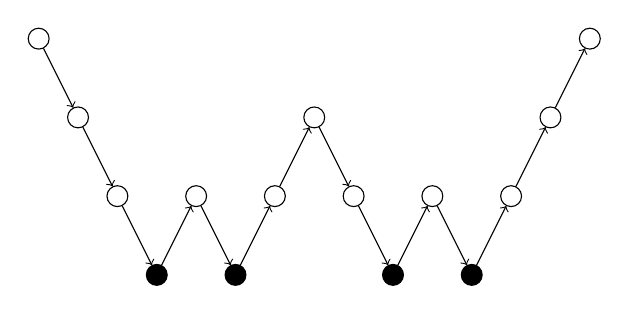
\begin{tikzpicture}
			\node	(a) at (0,4) [draw, circle,scale=0.8] {};
			\node	(b) at (0.5,3) [draw, circle,scale=0.8] {};
			\node	(c) at (1,2) [draw, circle,scale=0.8] {};
			\node	(d) at (1.5,1) [draw, circle,fill=black, scale=0.8] {};
			\node	(e) at (2,2) [draw, circle, scale=0.8] {};
			\node	(f) at (2.5,1) [draw, circle,fill=black,scale=0.8] {};
			\node	(g) at (3,2) [draw, circle,scale=0.8] {};
			\node	(h) at (3.5,3) [draw, circle,scale=0.8] {};
			\node	(i) at (4,2) [draw, circle,scale=0.8] {};
			\node	(j) at (4.5,1) [draw, circle,fill=black, scale=0.8] {};
			\node	(k) at (5,2) [draw, circle, scale=0.8] {};
			\node	(l) at (5.5,1) [draw, circle,fill=black,scale=0.8] {};
			\node	(m) at (6,2) [draw, circle,scale=0.8] {};
			\node	(n) at (6.5,3) [draw, circle, scale=0.8] {};
			\node	(o) at (7,4) [draw, circle, scale=0.8] {};
			
			\draw 
			(a) edge[->] (b) 
			(b) edge[->] (c)
			(c) edge[->] (d)
			(d) edge[->] (e)   
			(e) edge[->] (f)
			(f) edge[->] (g)
			(g) edge[->] (h)
			(h) edge[->] (i)
			(i) edge[->] (j)
			(j) edge[->] (k)
			(k) edge[->] (l)
			(l) edge[->] (m)
			(m) edge[->] (n)
			(n) edge[->] (o)
			;
		\end{tikzpicture}
		\subcaption*{$\gamma = 2$}
	\end{subfigure}
	\caption{Four-grid cycles ($l = 3$).}
	\label{fig:four-grid-cycles}
\end{figure}
Here each white node corresponds to one or multiple steps of smoothing on the respective level, while a black node implies that the resulting error equation is solved precisely.
Since, as it can be seen in Figure~\ref{fig:three-grid-cycles}, the choice of $\gamma = 1$ results in a V-shaped computational pattern, the corresponding multigrid method is usually called a V-cycle.
Similarly, the computational pattern of a method with $\gamma = 2$ on a three-grid hierarchy looks like a W, and hence the resulting method is called a W-cycle.
As it can be seen in Figure~\ref{fig:four-grid-cycles}, the amount of computational work within a W-cycle drastically increases with the number of coarsening steps.
While applying V-cycle always results in significantly fewer computations, in many cases, a single coarse grid correction step is not sufficient to reduce the low-frequency components of the initial error on the finest grid~\cite{trottenberg2000multigrid}.
Due to the resulting drastic increase in the number of computations, values of $\gamma$ larger than two are usually impractical for multigrid methods~\cite{trottenberg2000multigrid}.
While Algorithm~\ref{alg:multigrid-cycle} enables the construction of different multigrid methods based on choosing different values for the parameters $l$, $\gamma$, $\nu_1$, $\nu_2$ and $\omega$, the structural composition of the resulting methods is limited.
For instance, in Algorithm~\ref{alg:multigrid-cycle}, it is assumed that the same value of $\gamma$ is chosen on each level, which restricts possible computational patterns to those portrayed in Figure~\ref{fig:three-grid-cycles} and~\ref{fig:four-grid-cycles}.
One way to overcome this limitation is to combine different cycle types in a single method.
For instance, combining W- and V-cycles on each level results in a so-called F-cycle, whose algorithmic structure is illustrated by Figure~\ref{fig:f-cycle}.
\begin{figure}
	\begin{subfigure}{0.4\textwidth}
		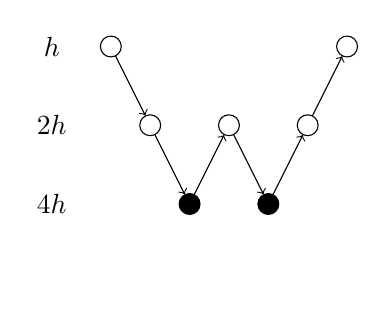
\begin{tikzpicture}
			\node   (h) at (-0.75, 4){$h$};
			\node   (2h) at (-0.75, 3){$2h$};
			\node   (4h) at (-0.75, 2){$4h$};
			\node   (8h) at (-0.75, 1){};
			\node	(a) at (0,4) [draw, circle,scale=0.8] {};
			\node	(b) at (0.5,3) [draw, circle,scale=0.8] {};
			\node	(c) at (1,2) [draw, circle,fill=black,scale=0.8] {};
			\node	(d) at (1.5,3) [draw, circle,scale=0.8] {};
			\node	(e) at (2,2) [draw, circle, fill=black, scale=0.8] {};
			\node	(f) at (2.5,3) [draw, circle, scale=0.8] {};
			\node	(g) at (3,4) [draw, circle, scale=0.8] {};
			
			\draw 
			(a) edge[->] (b) 
			(b) edge[->] (c)
			(c) edge[->] (d)
			(d) edge[->] (e)   
			(e) edge[->] (f)
			(f) edge[->] (g)
			;
		\end{tikzpicture}
	\end{subfigure}
	\begin{subfigure}{0.6\textwidth}
		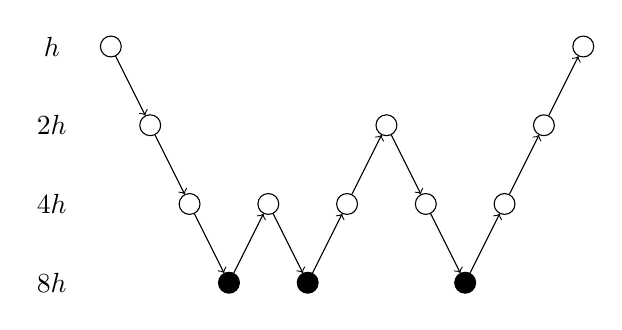
\begin{tikzpicture}
				\node   (h) at (-0.75, 4){$h$};
				\node   (2h) at (-0.75, 3){$2h$};
				\node   (4h) at (-0.75, 2){$4h$};
				\node   (8h) at (-0.75, 1){$8h$};
			\node	(a) at (0,4) [draw, circle,scale=0.8] {};
			\node	(b) at (0.5,3) [draw, circle,scale=0.8] {};
			\node	(c) at (1,2) [draw, circle,scale=0.8] {};
			\node	(d) at (1.5,1) [draw, circle,fill=black, scale=0.8] {};
			\node	(e) at (2,2) [draw, circle, scale=0.8] {};
			\node	(f) at (2.5,1) [draw, circle,fill=black,scale=0.8] {};
			\node	(g) at (3,2) [draw, circle,scale=0.8] {};
			\node	(h) at (3.5,3) [draw, circle,scale=0.8] {};
			\node	(i) at (4,2) [draw, circle,scale=0.8] {};
			\node	(j) at (4.5,1) [draw, circle,fill=black, scale=0.8] {};
			\node	(k) at (5,2) [draw, circle, scale=0.8] {};
			\node	(l) at (5.5,3) [draw, circle,scale=0.8] {};
			\node	(m) at (6,4) [draw, circle,scale=0.8] {};
			
			\draw 
			(a) edge[->] (b) 
			(b) edge[->] (c)
			(c) edge[->] (d)
			(d) edge[->] (e)   
			(e) edge[->] (f)
			(f) edge[->] (g)
			(g) edge[->] (h)
			(h) edge[->] (i)
			(i) edge[->] (j)
			(j) edge[->] (k)
			(k) edge[->] (l)
			(l) edge[->] (m)
			;
		\end{tikzpicture}
	\end{subfigure}
	\caption{Computational pattern of the F-cycle with a different number of coarsening steps.}
	\label{fig:f-cycle}
\end{figure}
Except for $l = 2$, in which case the F-cycle and W-cycle are equivalent, this method represents a compromise between a pure V-cycle and W-cycle.
While the composition of a multigrid method from different cycle types represents an additional degree of freedom, the individual cycles can still be formulated within the rules of Algorithm~\ref{alg:multigrid-cycle} and, hence, are fully described by the aforementioned parameters.
Since, according to the classical formulation of a multigrid method as in~\cite{brandt1977multi,hackbusch2013multi,trottenberg2000multigrid,briggs2000multigrid}, these parameters are considered global, adapting one of their values uniformly changes the method's behavior on each level. 
While for many applications, this approach has shown to yield efficient multigrid methods~\cite{trottenberg2000multigrid}, there are still cases where multigrid could not achieve its full potential~\cite{ernst2012difficult,benzi2005numerical}.
Even though, to date, there exists a rich amount of research on the optimization of multigrid cycles based on a fixed set of global parameters, the variation of its components on an individual level has not been considered yet.
Such an approach would grant the flexibility to generate multigrid cycles that consist of varying restriction and coarse-grid correction steps, each with a different combination of smoothers and relaxation factors.
In this work, we aim to realize this vision by expressing each multigrid cycle as a finite sequence of instructions whose order is restricted by the rules of linear algebra and multigrid theory.
To specify these rules in a mathematically formal way, we make use of programming language theory, such that the formulation of a multigrid method is treated as a program synthesis task.
In the next section, we, therefore, provide a brief overview of programming language theory and introduce the concept of formal languages and grammars.
We then combine this formalism together with our knowledge about multigrid methods to derive a novel representation of multigrid solvers that enables us to construct these methods in the form of a program design and optimization task.
  \section{Formal Languages and Grammars}
\label{sec:formal-languages}
In the previous section, we have introduced the theoretical background necessary to understand the fundamentals of multigrid methods.
The goal of this thesis is to develop a formal language that can express multigrid solvers of variable structure.
In general the \emph{alphabet} of a formal language is a non-empty set of symbols $\Sigma$.
Based on $\Sigma$ \emph{strings} can be created, which represent finite sequences of symbols.
For instance the alphabet $\Sigma = \left\{a, b\right\}$ contains only the symbols $a$ and $b$, as such $aabbb$ and $abaab$ are both strings on the alphabet $\Sigma$.
The length of a string, denoted by $|\cdot|$, is equal to the number of symbols contained in it. 
A concatenation of two strings 
\begin{equation}
	\begin{split}
		v & = a_1 a_2 \cdots a_n \\
		w & = b_1 b_2 \cdots b_m
	\end{split}
\end{equation}
is performed by appending the second string to the right of the first string such that
\begin{equation}
	vw = a_1 a_2 \cdots a_n b_1 b_2 \cdots b_m,
\end{equation}
The length of the concatenated string is then obviously equal to the sum of the length of the individual string, which means
\begin{equation}
|vw| = |v| + |w|.
\end{equation}
Finally, we define the empty string $\lambda$ as
\begin{equation}
	\begin{split}
		& |\lambda| = 0 \\
		& v \lambda = \lambda v = v,
	\end{split}
\end{equation}
where $v$ is a string on an arbitrary alphabet.
Assume $\Sigma$ is an alphabet, then $\Sigma^*$ is the set of strings obtained by concatenating zero or an arbitrary number of symbols from $\Sigma$.
Consequently, $\Sigma^*$ always contains the empty string $\lambda$.
To exclude $\lambda$ from the set, we define $\Sigma^+ = \Sigma^* \setminus \lambda$.
Since the number of strings that can be created from an alphabet through concatenation is infinite, both $\Sigma^+$ and $\Sigma^*$ represent infinite sets.
For example again let $\Sigma = \left\{a, b\right\}$ then
\begin{equation*}
	\Sigma^{*} = \left\{\lambda, a, b, aa, ab, ba, bb, aaa, aab, aba, \dots \right\}
\end{equation*} 
In general, for a given alphabet the \emph{language} $L$ is defined as a subset of $\Sigma^*$ (or $\Sigma^+$)
\begin{equation}
	L \supset \Sigma^*.
	\label{eq:language-basic-definition}
\end{equation}
However, in practice we usually want to obtain a language $L_G$ that represents a specific subset of $\Sigma^*$.
One way to achieve this is to define a set of rules that generate $L_G$.
These rules can be formally specified in form of a \emph{grammar}.
\begin{definition}[Grammar]
	\begin{equation*}
		G = \left(V, T, S, P \right),
	\end{equation*}
	where $V$ is a finite set of \emph{variables},
	$T$ a finite set of \emph{terminal symbols},
	$S \in V$ is the \emph{start} variable and 
	$P$ a finite set of \emph{productions} or \emph{production rules}.
	We also assume that $V \neq \emptyset$, $T \neq \emptyset$ and $V \cap T = \emptyset$.
\end{definition}
The core of a grammar are the productions $P$, which are usually specified as a set of mappings of the form
\begin{equation}
	x \to y,
	\label{eq:unrestricted-production}
\end{equation}
where $x \in \left(V \cup T\right)^+$ and $y \in \left(V \cup T\right)^*$.
Note that alternatively the operator
\begin{equation*}
	x \bnfpo y
\end{equation*}
is also often used to denote a production.
Each production rule $x \to y$ can then be applied in the following way.
Given a string $u$ of the form 
\begin{equation}
	u = vxw,
\end{equation}
we can replace $x$ with $y$ to \emph{derive} a new string
\begin{equation}
	u' = vyw,
\end{equation}
which is usually written as $u \Rightarrow u'$.
This process can then be continued by applying a sequence of derivations chosen arbitrarily from the set of available productions $P$.
Within this sequence each production can be applied whenever its conditions on the left-hand side of the rule are fulfilled, i.e. the respective pattern on occurs anywhere within the current string.
Also note that there is no limit on how many times a certain productions can be applied.
Each string $u$ at which we can arrive by applying an arbitrary sequence of productions starting from $S$
\begin{equation}
	S \Rightarrow \dots \Rightarrow u,
\end{equation}
is then an element of language $L_G$.
Assuming that 
\begin{equation}
	S \overset{*}{\Rightarrow} u.
\end{equation}
represents the application of an unspecified sequence of productions, we can define the language $L_G$ generated by the grammar $G$:
\begin{definition}[Language]\label{def:language}
	Let $G = \left\{V, T, S, P\right\}$ be a grammar, then
	\begin{equation}
		L_G = \left\{u \in T^* : S \overset{*}{\Rightarrow} u\right\}
	\end{equation}
is the language generated by $G$.
\end{definition}
Assuming $u \in L_G$ and 
\begin{equation}
	S \Rightarrow u_1 \Rightarrow u_2 \Rightarrow \dots \Rightarrow u_n \Rightarrow u
\end{equation}
is a \emph{derivation} of $u$, then the strings $S, u_1, u_2, \dots, u_n$ are called its \emph{sequential forms}.
\subsection{The Chomsky Hierarchy}
\label{sec:chomsky-hierarchy}
So far, we have not yet imposed any restrictions on the individual components of a grammar $G$.
We call such a grammar, whose productions are of the general form of Equation~\eqref{eq:unrestricted-production} \emph{unrestricted}.
In can be shown that any language generated by an unrestricted grammar is recursively enumerable, which means that there exists \emph{Turing machine} which is capable of enumerating all strings contained in that language~\cite{linz2006introduction}.
As a consequence, one can in fact prove that unrestricted grammars are equally powerful as Turing machines and, hence, both computational models are equivalent.
Since we are only interested in languages that possess this property and, hence, can be processed by any Turing-complete system on a modern computer, there is no use in considering languages that do not fall into this category.
While Turing machines and unrestricted grammars both represent an universal model of computation, it can be useful to consider grammars that impose certain restrictions on their productions and, hence, simplify both the derivation as well as the manipulation of strings.
\emph{Context-sensitive} grammars (CSG) represent a first step towards this direction.
\begin{definition}[Context-Sensitive Grammar]
A grammar $G = \left\{V, T, S, P\right\}$ is context-sensitive if all productions can be written as
\begin{equation*}
	xAy \to xuy
\end{equation*}
where $A \in V$ and $x, y, u \in \left(V \cup T\right)^*$.
\label{def:context-sensitive-grammar}
\end{definition}
This is equivalent to saying that a certain production $A \to u$ can only be peformed in the \emph{context} of $x$ and $y$, from which the term context-sensitive is derived.
While unrestricted grammars can be described by a Turing machine, the equivalent model of computation for a CSG is the \emph{linear bounded automaton}, which represents a Turing machine whose tape is linearly bounded by the length of the string~\cite{linz2006introduction}.
Furthermore, by prohibiting any context at the left-hand side of a production one arrives at the class of \emph{context-free} grammar (CFG).
\begin{definition}[Context-Free Grammar]
	A grammar $G = \left\{V, T, S, P\right\}$ is context-free if all productions are of the form
	\begin{equation*}
		A \to u 
	\end{equation*}
	where $A \in V$ and $u \in \left(V \cup T\right)^*$.
\end{definition}
The equivalent model of computation for a CFG is the \emph{pushdown automaton}~\cite{linz2006introduction}.  
CFGs have a number of desirable properties that justify their widespread use in computer science, especially in the theory of programming languages~\cite{pierce2002types}.
For instance, each string generated by a CFG as well as the derivation of each string can be represented as a tree.
Moreover, it is possible to check whether an arbitrary string of length $n$ is contained in the language generated by a CFG using only $\mathcal{O}(n^3)$ steps.
Note that the class of CFGs is contained in the class of CSGs, since we can simply replace each production 
\begin{equation}
	A \to u,
\end{equation}
of a CFG by one of the form
\begin{equation}
	xAy \to xuy,
\end{equation}
with $x = y = \lambda$. 
Since $\lambda \in \left(V \cup T\right)^*$, the resulting grammar meets the requirements of Definition~\ref{def:context-sensitive-grammar}.
Finally, the introduction of a further restriction on the productions leads to the class of regular grammars (RGs).
\begin{definition}[Regular Grammar]
	A grammar $G = \left\{V, T, S, P\right\}$ is regular if all productions are either of the form
	\begin{equation*}
		\begin{split}
			A & \to xB, \\
			A & \to x
		\end{split}
	\end{equation*}
in which case $G$ is said to be \emph{left-linear} or 
	\begin{equation*}
	\begin{split}
		A & \to Bx, \\
		A & \to x
	\end{split}
	\end{equation*}
in which case $G$ is said to be \emph{right-linear}, where in both cases $A, B \in V$ and $x \in T^*$.
\end{definition}
Since both $xB \in \left(V \cup T\right)^*$ and $Bx \in \left(V \cup T\right)^*$ it is obvious that each regular grammar can also be considered as a CFG.
Each language generated by a RG is a regular language and can, thus, be defined in form of a regular expression and, thus, they have the same expressive power as finite-state machines~\cite{linz2006introduction}.
With the definition of RGs we have arrived at the bottom of the so-called \emph{Chomsky hierarchy} of formal grammars and languages, which is given by the following set relations
\begin{equation*}
	\mathcal{G} \subset \mathcal{G}_{CS} \subset \mathcal{G}_{CF} \subset \mathcal{G}_{R}, 
\end{equation*} 
where $\mathcal{G}$ is the set of all unrestricted (type-0), $\mathcal{G}_{CS}$ the set of all context-sensitive (type-1), $\mathcal{G}_{CF}$ the set of all context-free (type-2) and $\mathcal{G}_{R}$ the set of all regular (type-3) grammars.
The same is true for the corresponding languages
\begin{equation*}
	\mathcal{L} \subset \mathcal{L}_{CS} \subset \mathcal{L}_{CF} \subset \mathcal{L}_{R}. 
\end{equation*}
Consequently, each level in this hierarchy corresponds to a particular class of grammars introduced in this section, where each subsequent level introduces further restrictions on the productions but on the other hand enables the use of faster and more efficient algorithms for manipulating the strings contained in its generated language.
After we have now introduced a class of formal languages for representing strings of symbols in a structured way as well as those grammars able to generate them, we next discuss how we can represent the construction and manipulation of such strings as a combinatorial search problem, whose solution we aim to approximate using randomized population-based search methods.







   


  \section{Genetic Programming}
\emph{Genetic Programming} (GP) is a class of search algorithms for finding optimal programs based on the principle of natural evolution first proposed by John Koza~\cite{koza1994genetic}.
In general, a program $p$ can be considered as a mapping from the set of inputs $\mathcal{I}$ to the corresponding set of outputs $\mathcal{O}$
\begin{equation}
	p : \mathcal{I} \to \mathcal{O}.
\end{equation}
However, since not all input-output pairs are known in advance, this mapping is usually given in form of a finite set of training cases.
The goal of GP is then to find a program that correctly computes the correct output for each input contained in the training set.
Since there is often not a unique program that satisfies this condition, usually a number of additional constraints are applied to assess the quality of each correct program.
For instance, in practice one is often interested in finding the shortest or fastest program that is able to pass all training cases.
Based on a program's effectiveness in solving all training cases under the given constraints, GP then assigns a \emph{fitness} value to each program, which is then treated as an \emph{individual} within a \emph{population} of programs.
In evolutionary computation, the population is a set of individuals currently considered within the search and, therefore, spans a subspace within the space of solutions for the given search problem.
Each subsequent step of the search is then performed by generating a new population based on the previous one through \emph{mutation} or recombination (often called \emph{crossover}) of the individuals contained in the current one.
Usually, the candidates for mutation and crossover are sampled from the current population based on the fitness value computed for each individual.
If we repeat this procedure for a number of $n$ steps, we arrive at a final population $P_n$, which can then additionally be evaluated on a test set, to obtain the best overall program.
The resulting search method is summarized in Algorithm~\ref{alg:genetic-programming}. 
\begin{algorithm}[t]
	\caption{Genetic Programming}
	\label{alg:genetic-programming}
	\begin{algorithmic} % The number tells where the line numbering should start
		\State \textbf{Randomly generate} an initial population $P_0$ of programs
		\State \textbf{Evaluate} $P_0$ on the \textbf{training set} 
		\For{$i := 1, \dots, n$}
		\State \textbf{Select} a subset of individuals $M_i \supset P_{i-1}$ based on their \textbf{fitness}
		\State \textbf{Generate} new programs $C_i$ based on $M_i$ using \textbf{mutation} and \textbf{crossover}
		\State \textbf{Evaluate} $C_i$ on the \textbf{training set} 
		\State \textbf{Select} $P_{i}$ from $C_i \cup P_{i-1}$
		\EndFor
		\State \textbf{Evaluate} the final population $P_{n}$ on a \textbf{test set}  to obtain the best overall program
	\end{algorithmic}
\end{algorithm}
While Algorithm~\ref{alg:genetic-programming} gives an overview of the general structure of a GP method, we have not yet considered how the individual operations such as the generation of an initial population and the creation of new individuals through mutation and crossover can be performed.
Since all these operations are based on manipulating the internal structure of a given program, the first step in the implementation of a GP method choosing a suitable program representation.
Note that this representation does not necessarily need to be equal to the target language in which the actual program is supposed to be implemented but rather needs to define a unique mapping that enables its automatic generation.
This process is usually called \emph{genotype} to \emph{phenotype} mapping, where the genotype refers to the internal representation used within GP while the phenotype then represents the actual program implemented on the target machine.
One of the most widely used genotype representations is tree-based GP, where each program is internally represented as a tree of expressions, which was also initially proposed by John Koza~\cite{koza1994genetic}.
While within the last decades numerous other GP variants have been proposed~\cite{poli2008field}, such as grammatical evolution~\cite{o2001grammatical}, linear GP~\cite{brameier2007linear} and cartesian GP~\cite{miller2008cartesian}, we focus on tree-based GP as it forms the basis for our implementation, which will be presented in later chapters.
\section{Representation}
In contrast to other evolutionary algorithms algorithms, which usually represent the solution to an optimization problem as an array of discrete or continuous numbers~\cite{back1997handbook}, GP deals with the optimization of programs and, hence, each solution corresponds to an executable program.
%Before we consider these operations in detail, we first need to define a procedure to generate program expression trees in a structured way. 
For this purpose, we consider the following context-free grammar $G$ with the productions
\begin{equation}
	\begin{split}
		S & \to E \\
		E & \to \text{if} \; B \; \text{then} \; E \; \text{else} \; E \; | \; A \\
		A & \to -A \; | \; (A + A) \; | \; (A - A) \; | \; (A \cdot A) \; | \; A^A \; | \; x \; | \; y \\  
		B & \to \neg B \; | \; (B \wedge B) \; | \; (B \vee B) \; | \; u \; | \; v,
	\end{split}
\label{eq:gp-example-grammar}
\end{equation}
where $V = \{S, E, A, B\}$ is the set of variables and the symbols $x$, $y$ represent numbers while the symbols $u$, $v$ correspond to boolean values, i.e. $\top$ or $\bot$.
If we treat $x$, $y$, $u$ and $v$ as an input, each expression generated by $G$ can be considered as a quaternary function $f(x,y,u,v) \in L_{G}$, where $L_G$ is the language generated by $G$ according to Definition~\ref{def:language}.
For example the functions
\begin{equation}
	\begin{split}
		f_1(x,y,u,v) & = \text{if} \; (\neg u \wedge v) \; \text{then} \; (x \cdot x) \; \text{else} \; (x / y) \\
		f_2(x,y,u,v) & = x^{(x + y)} - (y \cdot y)
	\end{split}
\label{eq:gp-example-functions}
\end{equation} can both be generated by $G$ and are, hence, included in $L_G$.
By applying the rules of arithmetic and boolean algebra, we can compute the result of each such function based on a given set of inputs.
Therefore, assuming both $x$ and $y$ represent real-valued numbers, we can evaluate the correctness of the mapping $f : x, y, u, v \to \mathbb{R}$ for an arbitrary number of test cases.
Next, to define suitable operations for generating arbitrary functions $f \in L_G$, we need to choose a suitable data structure for its representation.
While a program's structure depends on the programming language it is formulated in, in many cases it is possible to formulate it as a tree of program expressions, which is especially true for languages from the Lisp-family, that have been originally employed in John Koza's work~\cite{koza1994genetic}.
In tree-based GP all operations are performed on program expression trees and, thus, both mutation and crossover must be designed with respect to this representation.
Expression trees can be created in a straightforward way after rewriting each expression in postfix notation. 
To obtain the corresponding tree, the expressions is traversed sequentially by putting each operand that either represents a terminal symbol or has been already transformed on a stack and then retrieving those operands from the top of the stack for each new operator encountered.
Figure~\ref{fig:gp-expression-tree-examples} shows the corresponding expression trees for $f_1$ and $f_2$.
\begin{figure}
	\begin{subfigure}{0.59\textwidth}
		\includegraphics{figures/gp_tree1.pdf}
	\end{subfigure}
	\begin{subfigure}{0.41\textwidth}
		\includegraphics{figures/gp_tree2.pdf}
	\end{subfigure}
 \caption{Expression trees for $f_1$ and $f_2$, where we have simplified the if-then-else construct to a single ternary operator.}
 \label{fig:gp-expression-tree-examples}
\end{figure}
On the other hand, given a certain expression tree, we can easily restore the original expression by traversing the tree recursively in a top-down manner while generating the corresponding expression for each node as soon as each of its operands has been recursively processed or in case it is available as a terminal symbol.
While expression trees can be both easily generated from a given program, as well as offering an efficient way to evaluate a certain program, they possess an inherent limitation, which is the absence of type information.
For a better understanding of this, we reconsider the context-free grammar formulated in Equation~\eqref{eq:gp-example-grammar}.
Therein all productions on the variable $B$ only result in the generation of boolean expressions, while all productions starting from $A$ exclusively lead to arithmetic expressions.
As a consequence, we are not allowed to intermix expressions that are derived from $A$ and $B$.
However, this information is not contained in any of the expressions generated by $G$ and, hence, also missing in the corresponding tree.
As the generation of each new expression can be performed based on the productions of $G$, it is guaranteed to be valid.
However, the main step of GP is the creation of new individuals based on the existing ones in the population either through recombination of two individuals (crossover) or by altering certain parts of a given individual (mutation). 
Both operations require us to investigate which nodes and subtrees of a given expression trees can be safely replaced by an alternative branch without violating the type constraints imposed within the productions of our grammar.
While it is possible to deal with this problem by simply evicting those individuals that violate any type constraints from the population, depending on the number of constraints, this will be the case for a high percentage of individuals, leading to a highly inefficient method.
A different and usually more efficient approach is to annotate each node within an expression tree with additional type information, which leads to the concept of strongly-typed GP, first proposed by David Montana~\cite{montana1995strongly}.
Strongly-typed GP represents a viable solution to the problem of retaining type correctness, but it requires us to transform the implicit type information contained within the productions of our grammar into explicit type annotations at the nodes of each expression tree.
As an alternative we can instead utilize the information encoded in the productions of a grammar $G$ by considering the \emph{derivations} of an expression $e \in L_G$, as defined by
\begin{equation}
	S \Rightarrow e_1 \Rightarrow e_2 \Rightarrow \dots \Rightarrow e_n \Rightarrow e.
\end{equation}
If $G$ is context-free each of its possible derivations can be represented as a tree, where the root node is always the start variable $S$ and each level of the tree corresponds to a sequential form $e_i$ within the derivation~\cite{linz2006introduction}.
%Furthermore, if $G$ is regular, its derivations can be further simplified to finite state machine, where each state corresponds to a sequential form. 

  % TODO currently dummy file Unfortunately, determining the spectral radius requires the computation of the eigenvalues of a matrix $G$, which, in general, is of complexity $\mathcal{O}(n^3)$ for $G \in \mathbb{R}^{n \times n}$~\cite{demmel2007fast}.
In cases where the system of linear equations is obtained from the discretization of PDEs on a regular grid with uniform spacing and thus where the matrix $G$ is available in form of one or multiple stencil codes, it is possible to employ local Fourier analysis (LFA)~\cite{wienands2004practical}.
LFA considers a reformulation of the given problem on an infinite grid, which is transferred to the frequency domain to investigate the symbol of the underlying operator.
Based on the latter, an estimation of the spectral radius can then be computed in significantly less time.






% start the appendix (arabic page numbering [continued],
% uppercase alphabetic sectioning numbering, header)
\appendix 
  
  %%% WRITE YOUR APPENDIX DIRECTLY HERE OR %%%%%%%%
  %%% INPUT AN EXTERNAL FILE WITH YOUR APPENDIX %%%
  %\blinddocument

    
% start the backmatter (arabic page numbering [continued],
% no sectioning numbering, header)
\backmatter
  \bibliographystyle{abbrv}
  %TODO fix faupress bibliography
  % typeset the bibliography, settings can be
  % tweaked via the class option bibliography
  % \faupressprintbibliography
  \bibliography{bibliography}

\end{document}
